\documentclass[1p]{elsarticle_modified}
%\bibliographystyle{elsarticle-num}

%\usepackage[colorlinks]{hyperref}
%\usepackage{abbrmath_seonhwa} %\Abb, \Ascr, \Acal ,\Abf, \Afrak
\usepackage{amsfonts}
\usepackage{amssymb}
\usepackage{amsmath}
\usepackage{amsthm}
\usepackage{scalefnt}
\usepackage{amsbsy}
\usepackage{kotex}
\usepackage{caption}
\usepackage{subfig}
\usepackage{color}
\usepackage{graphicx}
\usepackage{xcolor} %% white, black, red, green, blue, cyan, magenta, yellow
\usepackage{float}
\usepackage{setspace}
\usepackage{hyperref}

\usepackage{tikz}
\usetikzlibrary{arrows}

\usepackage{multirow}
\usepackage{array} % fixed length table
\usepackage{hhline}

%%%%%%%%%%%%%%%%%%%%%
\makeatletter
\renewcommand*\env@matrix[1][\arraystretch]{%
	\edef\arraystretch{#1}%
	\hskip -\arraycolsep
	\let\@ifnextchar\new@ifnextchar
	\array{*\c@MaxMatrixCols c}}
\makeatother %https://tex.stackexchange.com/questions/14071/how-can-i-increase-the-line-spacing-in-a-matrix
%%%%%%%%%%%%%%%

\usepackage[normalem]{ulem}

\newcommand{\msout}[1]{\ifmmode\text{\sout{\ensuremath{#1}}}\else\sout{#1}\fi}
%SOURCE: \msout is \stkout macro in https://tex.stackexchange.com/questions/20609/strikeout-in-math-mode

\newcommand{\cancel}[1]{
	\ifmmode
	{\color{red}\msout{#1}}
	\else
	{\color{red}\sout{#1}}
	\fi
}

\newcommand{\add}[1]{
	{\color{blue}\uwave{#1}}
}

\newcommand{\replace}[2]{
	\ifmmode
	{\color{red}\msout{#1}}{\color{blue}\uwave{#2}}
	\else
	{\color{red}\sout{#1}}{\color{blue}\uwave{#2}}
	\fi
}

\newcommand{\Sol}{\mathcal{S}} %segment
\newcommand{\D}{D} %diagram
\newcommand{\A}{\mathcal{A}} %arc


%%%%%%%%%%%%%%%%%%%%%%%%%%%%%5 test

\def\sl{\operatorname{\textup{SL}}(2,\Cbb)}
\def\psl{\operatorname{\textup{PSL}}(2,\Cbb)}
\def\quan{\mkern 1mu \triangleright \mkern 1mu}

\theoremstyle{definition}
\newtheorem{thm}{Theorem}[section]
\newtheorem{prop}[thm]{Proposition}
\newtheorem{lem}[thm]{Lemma}
\newtheorem{ques}[thm]{Question}
\newtheorem{cor}[thm]{Corollary}
\newtheorem{defn}[thm]{Definition}
\newtheorem{exam}[thm]{Example}
\newtheorem{rmk}[thm]{Remark}
\newtheorem{alg}[thm]{Algorithm}

\newcommand{\I}{\sqrt{-1}}
\begin{document}

%\begin{frontmatter}
%
%\title{Boundary parabolic representations of knots up to 8 crossings}
%
%%% Group authors per affiliation:
%\author{Yunhi Cho} 
%\address{Department of Mathematics, University of Seoul, Seoul, Korea}
%\ead{yhcho@uos.ac.kr}
%
%
%\author{Seonhwa Kim} %\fnref{s_kim}}
%\address{Center for Geometry and Physics, Institute for Basic Science, Pohang, 37673, Korea}
%\ead{ryeona17@ibs.re.kr}
%
%\author{Hyuk Kim}
%\address{Department of Mathematical Sciences, Seoul National University, Seoul 08826, Korea}
%\ead{hyukkim@snu.ac.kr}
%
%\author{Seokbeom Yoon}
%\address{Department of Mathematical Sciences, Seoul National University, Seoul, 08826,  Korea}
%\ead{sbyoon15@snu.ac.kr}
%
%\begin{abstract}
%We find all boundary parabolic representation of knots up to 8 crossings.
%
%\end{abstract}
%\begin{keyword}
%    \MSC[2010] 57M25 
%\end{keyword}
%
%\end{frontmatter}

%\linenumbers
%\tableofcontents
%
\newcommand\colored[1]{\textcolor{white}{\rule[-0.35ex]{0.8em}{1.4ex}}\kern-0.8em\color{red} #1}%
%\newcommand\colored[1]{\textcolor{white}{ #1}\kern-2.17ex	\textcolor{white}{ #1}\kern-1.81ex	\textcolor{white}{ #1}\kern-2.15ex\color{red}#1	}

{\Large $\underline{12a_{0119}~(K12a_{0119})}$}

\setlength{\tabcolsep}{10pt}
\renewcommand{\arraystretch}{1.6}
\vspace{1cm}\begin{tabular}{m{100pt}>{\centering\arraybackslash}m{274pt}}
\multirow{5}{120pt}{
	\centering
	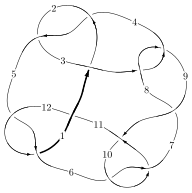
\includegraphics[width=112pt]{../../../GIT/diagram.site/Diagrams/png/920_12a_0119.png}\\
\ \ \ A knot diagram\footnotemark}&
\allowdisplaybreaks
\textbf{Linearized knot diagam} \\
\cline{2-2}
 &
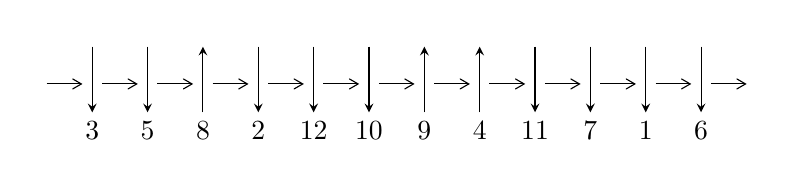
\begin{tikzpicture}[x=20pt, y=17pt]
	% nodes
	\node (C0) at (0, 0) {};
	\node (C1) at (1, 0) {};
	\node (C1U) at (1, +1) {};
	\node (C1D) at (1, -1) {3};

	\node (C2) at (2, 0) {};
	\node (C2U) at (2, +1) {};
	\node (C2D) at (2, -1) {5};

	\node (C3) at (3, 0) {};
	\node (C3U) at (3, +1) {};
	\node (C3D) at (3, -1) {8};

	\node (C4) at (4, 0) {};
	\node (C4U) at (4, +1) {};
	\node (C4D) at (4, -1) {2};

	\node (C5) at (5, 0) {};
	\node (C5U) at (5, +1) {};
	\node (C5D) at (5, -1) {12};

	\node (C6) at (6, 0) {};
	\node (C6U) at (6, +1) {};
	\node (C6D) at (6, -1) {10};

	\node (C7) at (7, 0) {};
	\node (C7U) at (7, +1) {};
	\node (C7D) at (7, -1) {9};

	\node (C8) at (8, 0) {};
	\node (C8U) at (8, +1) {};
	\node (C8D) at (8, -1) {4};

	\node (C9) at (9, 0) {};
	\node (C9U) at (9, +1) {};
	\node (C9D) at (9, -1) {11};

	\node (C10) at (10, 0) {};
	\node (C10U) at (10, +1) {};
	\node (C10D) at (10, -1) {7};

	\node (C11) at (11, 0) {};
	\node (C11U) at (11, +1) {};
	\node (C11D) at (11, -1) {1};

	\node (C12) at (12, 0) {};
	\node (C12U) at (12, +1) {};
	\node (C12D) at (12, -1) {6};
	\node (C13) at (13, 0) {};

	% arrows
	\draw[->,>={angle 60}]
	(C0) edge (C1) (C1) edge (C2) (C2) edge (C3) (C3) edge (C4) (C4) edge (C5) (C5) edge (C6) (C6) edge (C7) (C7) edge (C8) (C8) edge (C9) (C9) edge (C10) (C10) edge (C11) (C11) edge (C12) (C12) edge (C13) ;	\draw[->,>=stealth]
	(C1U) edge (C1D) (C2U) edge (C2D) (C3D) edge (C3U) (C4U) edge (C4D) (C5U) edge (C5D) (C6U) edge (C6D) (C7D) edge (C7U) (C8D) edge (C8U) (C9U) edge (C9D) (C10U) edge (C10D) (C11U) edge (C11D) (C12U) edge (C12D) ;
	\end{tikzpicture} \\
\hhline{~~} \\& 
\textbf{Solving Sequence} \\ \cline{2-2} 
 &
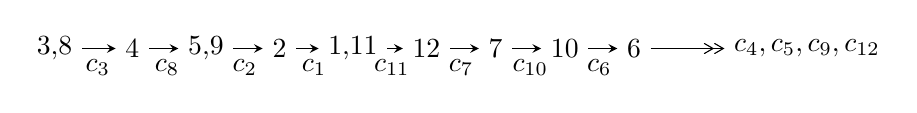
\begin{tikzpicture}[x=25pt, y=7pt]
	% node
	\node (A0) at (-1/8, 0) {3,8};
	\node (A1) at (1, 0) {4};
	\node (A2) at (33/16, 0) {5,9};
	\node (A3) at (25/8, 0) {2};
	\node (A4) at (67/16, 0) {1,11};
	\node (A5) at (21/4, 0) {12};
	\node (A6) at (25/4, 0) {7};
	\node (A7) at (29/4, 0) {10};
	\node (A8) at (33/4, 0) {6};
	\node (C1) at (1/2, -1) {$c_{3}$};
	\node (C2) at (3/2, -1) {$c_{8}$};
	\node (C3) at (21/8, -1) {$c_{2}$};
	\node (C4) at (29/8, -1) {$c_{1}$};
	\node (C5) at (19/4, -1) {$c_{11}$};
	\node (C6) at (23/4, -1) {$c_{7}$};
	\node (C7) at (27/4, -1) {$c_{10}$};
	\node (C8) at (31/4, -1) {$c_{6}$};
	\node (A9) at (43/4, 0) {$c_{4},c_{5},c_{9},c_{12}$};

	% edge
	\draw[->,>=stealth]	
	(A0) edge (A1) (A1) edge (A2) (A2) edge (A3) (A3) edge (A4) (A4) edge (A5) (A5) edge (A6) (A6) edge (A7) (A7) edge (A8) ;
	\draw[->>,>={angle 60}]	
	(A8) edge (A9);
\end{tikzpicture} \\ 

\end{tabular} \\

\footnotetext{
The image of knot diagram is generated by the software ``\textbf{Draw programme}" developed by Andrew Bartholomew(\url{http://www.layer8.co.uk/maths/draw/index.htm\#Running-draw}), where we modified some parts for our purpose(\url{https://github.com/CATsTAILs/LinksPainter}).
}\phantom \\ \newline 
\centering \textbf{Ideals for irreducible components\footnotemark of $X_{\text{par}}$} 
 
\begin{align*}
I^u_{1}&=\langle 
2 u^{13}- u^{11}+2 u^{10}+5 u^9+2 u^8+2 u^7-4 u^6+3 u^5+2 u^4-2 u^3-12 u^2+4 d-8 u-8,\\
\phantom{I^u_{1}}&\phantom{= \langle  }- u^{13}+u^{11}- u^{10}-4 u^9+u^8+u^7-4 u^5- u^4+2 u^3+8 u^2+4 c+4,\\
\phantom{I^u_{1}}&\phantom{= \langle  }- u^{13}+u^{11}- u^{10}-3 u^9+u^7+u^6-2 u^5- u^4+2 u^3+6 u^2+2 b+2 u+2,\\
\phantom{I^u_{1}}&\phantom{= \langle  }3 u^{13}-2 u^{11}+3 u^{10}+9 u^9+u^8- u^7-4 u^6+7 u^5+3 u^4-6 u^3-18 u^2+4 a-8 u-12,\\
\phantom{I^u_{1}}&\phantom{= \langle  }u^{14}- u^{13}- u^{12}+2 u^{11}+2 u^{10}-3 u^9- u^8- u^7+4 u^6- u^5-4 u^4-4 u^3+4 u^2+4\rangle \\
I^u_{2}&=\langle 
-3 u^{21}+9 u^{19}+\cdots+4 d+4,\;-2 u^{22}+6 u^{20}+\cdots+4 c-2,\\
\phantom{I^u_{2}}&\phantom{= \langle  }- u^{16}+2 u^{14}-5 u^{12}+6 u^{10}- u^9-6 u^8+u^7+4 u^6-4 u^5- u^4+3 u^3-4 u^2+2 b-2 u,\\
\phantom{I^u_{2}}&\phantom{= \langle  }-2 u^{21}+4 u^{20}+\cdots+4 a+6,\;u^{23}-2 u^{22}+\cdots+2 u-2\rangle \\
I^u_{3}&=\langle 
-3 u^{21}+9 u^{19}+\cdots+4 d+4,\;-2 u^{22}+6 u^{20}+\cdots+4 c-2,\;2 u^{22}-2 u^{21}+\cdots+4 b+2,\\
\phantom{I^u_{3}}&\phantom{= \langle  }-2 u^{22}+u^{21}+\cdots+4 a-6,\;u^{23}-2 u^{22}+\cdots+2 u-2\rangle \\
I^u_{4}&=\langle 
-2 u^{22}+3 u^{21}+\cdots+4 d+10 u,\;u^{19}-2 u^{17}+\cdots+4 c+4,\;2 u^{22}-2 u^{21}+\cdots+4 b+2,\\
\phantom{I^u_{4}}&\phantom{= \langle  }-2 u^{22}+u^{21}+\cdots+4 a-6,\;u^{23}-2 u^{22}+\cdots+2 u-2\rangle \\
I^u_{5}&=\langle 
- a^2 u^2 c- u^2 c a+2 a^2 u^2- a^2 c+2 c a u+2 u^2 a+4 c a-3 c u+a u- u^2+d-4 c-5 a+u+3,\\
\phantom{I^u_{5}}&\phantom{= \langle  }a^2 u^2 c- a^2 c u+3 u^2 c a-2 a^2 u^2- a^2 c+4 c a u-2 u^2 c- u^2 a+c^2- c a-2 c u+2 a^2-5 a u+2 a+3 u-1,\\
\phantom{I^u_{5}}&\phantom{= \langle  }- a^2 u^2+b+2 a-2,\;a^3-2 a^2 u-2 a^2+3 a u+3 a- u-1,\;u^3+u^2-1\rangle \\
\\
I^v_{1}&=\langle 
a,\;d,\;c+1,\;b-1,\;v+1\rangle \\
I^v_{2}&=\langle 
c,\;d+1,\;b,\;a-1,\;v+1\rangle \\
I^v_{3}&=\langle 
a,\;d+1,\;c+a,\;b-1,\;v+1\rangle \\
I^v_{4}&=\langle 
a,\;d a- c+1,\;d v-1,\;c v- a- v,\;b-1\rangle \\
\end{align*}
\raggedright * 8 irreducible components of $\dim_{\mathbb{C}}=0$, with total 104 representations.\\
\raggedright * 1 irreducible components of $\dim_{\mathbb{C}}=1$ \\
\footnotetext{All coefficients of polynomials are rational numbers. But the coefficients are sometimes approximated in decimal forms when there is not enough margin.}
\newpage
\renewcommand{\arraystretch}{1}
\centering \section*{I. $I^u_{1}= \langle 2 u^{13}- u^{11}+\cdots+4 d-8,\;- u^{13}+u^{11}+\cdots+4 c+4,\;- u^{13}+u^{11}+\cdots+2 b+2,\;3 u^{13}-2 u^{11}+\cdots+4 a-12,\;u^{14}- u^{13}+\cdots+4 u^2+4 \rangle$}
\flushleft \textbf{(i) Arc colorings}\\
\begin{tabular}{m{7pt} m{180pt} m{7pt} m{180pt} }
\flushright $a_{3}=$&$\begin{pmatrix}1\\0\end{pmatrix}$ \\
\flushright $a_{8}=$&$\begin{pmatrix}0\\u\end{pmatrix}$ \\
\flushright $a_{4}=$&$\begin{pmatrix}1\\- u^2\end{pmatrix}$ \\
\flushright $a_{5}=$&$\begin{pmatrix}-\frac{3}{4} u^{13}+\frac{1}{2} u^{11}+\cdots+2 u+3\\\frac{1}{2} u^{13}-\frac{1}{2} u^{11}+\cdots- u-1\end{pmatrix}$ \\
\flushright $a_{9}=$&$\begin{pmatrix}u\\- u^3+u\end{pmatrix}$ \\
\flushright $a_{2}=$&$\begin{pmatrix}-\frac{3}{4} u^{13}+\frac{1}{2} u^{11}+\cdots+2 u+3\\\frac{1}{2} u^{13}-\frac{1}{4} u^{11}+\cdots-2 u-2\end{pmatrix}$ \\
\flushright $a_{1}=$&$\begin{pmatrix}-\frac{1}{4} u^{13}+\frac{1}{4} u^{11}+\cdots+\frac{3}{2} u^2+1\\\frac{1}{2} u^{13}-\frac{1}{4} u^{11}+\cdots-2 u-2\end{pmatrix}$ \\
\flushright $a_{11}=$&$\begin{pmatrix}\frac{1}{4} u^{13}-\frac{1}{4} u^{11}+\cdots-2 u^2-1\\-\frac{1}{2} u^{13}+\frac{1}{4} u^{11}+\cdots+2 u+2\end{pmatrix}$ \\
\flushright $a_{12}=$&$\begin{pmatrix}\frac{1}{2} u^{13}-\frac{1}{2} u^{11}+\cdots- u-2\\-\frac{1}{2} u^{13}-\frac{1}{2} u^{10}+\cdots+2 u+2\end{pmatrix}$ \\
\flushright $a_{7}=$&$\begin{pmatrix}- u^3\\u^5- u^3+u\end{pmatrix}$ \\
\flushright $a_{10}=$&$\begin{pmatrix}-\frac{1}{4} u^{13}+\frac{1}{4} u^{11}+\cdots+2 u+1\\\frac{1}{4} u^{11}-\frac{1}{4} u^9+\cdots-\frac{3}{2} u^3+u\end{pmatrix}$ \\
\flushright $a_{6}=$&$\begin{pmatrix}-\frac{3}{4} u^{13}+\frac{1}{2} u^{11}+\cdots+2 u+3\\\frac{1}{2} u^{13}-\frac{1}{2} u^{11}+\cdots- u-1\end{pmatrix}$\\&\end{tabular}
\flushleft \textbf{(ii) Obstruction class $= -1$}\\~\\
\flushleft \textbf{(iii) Cusp Shapes $= -3 u^{13}- u^{12}+u^{11}-2 u^{10}-8 u^9-5 u^8-3 u^7+7 u^6-2 u^5-7 u^4+4 u^3+22 u^2+16 u+10$}\\~\\
\newpage\renewcommand{\arraystretch}{1}
\flushleft \textbf{(iv) u-Polynomials at the component}\newline \\
\begin{tabular}{m{50pt}|m{274pt}}
Crossings & \hspace{64pt}u-Polynomials at each crossing \\
\hline $$\begin{aligned}c_{1},c_{9},c_{11}\end{aligned}$$&$\begin{aligned}
&u^{14}+7 u^{13}+\cdots+3 u+1
\end{aligned}$\\
\hline $$\begin{aligned}c_{2},c_{4},c_{5}\\c_{6},c_{10},c_{12}\end{aligned}$$&$\begin{aligned}
&u^{14}- u^{13}+\cdots+u+1
\end{aligned}$\\
\hline $$\begin{aligned}c_{3},c_{8}\end{aligned}$$&$\begin{aligned}
&u^{14}+u^{13}+\cdots+4 u^2+4
\end{aligned}$\\
\hline $$\begin{aligned}c_{7}\end{aligned}$$&$\begin{aligned}
&u^{14}-3 u^{13}+\cdots+32 u+16
\end{aligned}$\\
\hline
\end{tabular}\\~\\
\newpage\renewcommand{\arraystretch}{1}
\flushleft \textbf{(v) Riley Polynomials at the component}\newline \\
\begin{tabular}{m{50pt}|m{274pt}}
Crossings & \hspace{64pt}Riley Polynomials at each crossing \\
\hline $$\begin{aligned}c_{1},c_{9},c_{11}\end{aligned}$$&$\begin{aligned}
&y^{14}+5 y^{13}+\cdots+9 y+1
\end{aligned}$\\
\hline $$\begin{aligned}c_{2},c_{4},c_{5}\\c_{6},c_{10},c_{12}\end{aligned}$$&$\begin{aligned}
&y^{14}-7 y^{13}+\cdots-3 y+1
\end{aligned}$\\
\hline $$\begin{aligned}c_{3},c_{8}\end{aligned}$$&$\begin{aligned}
&y^{14}-3 y^{13}+\cdots+32 y+16
\end{aligned}$\\
\hline $$\begin{aligned}c_{7}\end{aligned}$$&$\begin{aligned}
&y^{14}+9 y^{13}+\cdots-1536 y+256
\end{aligned}$\\
\hline
\end{tabular}\\~\\
\newpage\flushleft \textbf{(vi) Complex Volumes and Cusp Shapes}
$$\begin{array}{c|c|c}  
\text{Solutions to }I^u_{1}& \I (\text{vol} + \sqrt{-1}CS) & \text{Cusp shape}\\
 \hline 
\begin{aligned}
u &= -0.351654 + 0.974470 I \\
a &= \phantom{-}0.484407 + 0.125788 I \\
b &= \phantom{-}0.933970 - 0.502203 I \\
c &= \phantom{-}0.065921 - 0.250683 I \\
d &= -0.762746 - 0.668204 I\end{aligned}
 & -2.00841 + 5.97343 I & -8.41754 - 8.60965 I \\ \hline\begin{aligned}
u &= -0.351654 - 0.974470 I \\
a &= \phantom{-}0.484407 - 0.125788 I \\
b &= \phantom{-}0.933970 + 0.502203 I \\
c &= \phantom{-}0.065921 + 0.250683 I \\
d &= -0.762746 + 0.668204 I\end{aligned}
 & -2.00841 - 5.97343 I & -8.41754 + 8.60965 I \\ \hline\begin{aligned}
u &= -0.915559 + 0.598258 I \\
a &= \phantom{-}0.664888 - 0.608266 I \\
b &= -0.181237 + 0.749038 I \\
c &= -1.159390 + 0.550105 I \\
d &= -0.936616 - 0.512222 I\end{aligned}
 & \phantom{-}0.94494 - 2.29172 I & -1.04510 + 1.71019 I \\ \hline\begin{aligned}
u &= -0.915559 - 0.598258 I \\
a &= \phantom{-}0.664888 + 0.608266 I \\
b &= -0.181237 - 0.749038 I \\
c &= -1.159390 - 0.550105 I \\
d &= -0.936616 + 0.512222 I\end{aligned}
 & \phantom{-}0.94494 + 2.29172 I & -1.04510 - 1.71019 I \\ \hline\begin{aligned}
u &= \phantom{-}1.120580 + 0.015323 I \\
a &= \phantom{-}0.577432 - 1.267280 I \\
b &= -0.702265 + 0.653431 I \\
c &= \phantom{-}0.530358 + 0.435838 I \\
d &= -0.072651 - 0.949218 I\end{aligned}
 & \phantom{-}4.01770 + 3.65190 I & -0.27967 - 6.51151 I \\ \hline\begin{aligned}
u &= \phantom{-}1.120580 - 0.015323 I \\
a &= \phantom{-}0.577432 + 1.267280 I \\
b &= -0.702265 - 0.653431 I \\
c &= \phantom{-}0.530358 - 0.435838 I \\
d &= -0.072651 + 0.949218 I\end{aligned}
 & \phantom{-}4.01770 - 3.65190 I & -0.27967 + 6.51151 I\\
 \hline 
 \end{array}$$\newpage$$\begin{array}{c|c|c}  
\text{Solutions to }I^u_{1}& \I (\text{vol} + \sqrt{-1}CS) & \text{Cusp shape}\\
 \hline 
\begin{aligned}
u &= -1.145230 + 0.485598 I \\
a &= -0.08828 + 1.64061 I \\
b &= -1.032700 - 0.607770 I \\
c &= \phantom{-}0.834303 + 0.325183 I \\
d &= -0.546866 - 0.244514 I\end{aligned}
 & \phantom{-}0.82935 - 11.25490 I & -6.02298 + 10.89166 I \\ \hline\begin{aligned}
u &= -1.145230 - 0.485598 I \\
a &= -0.08828 - 1.64061 I \\
b &= -1.032700 + 0.607770 I \\
c &= \phantom{-}0.834303 - 0.325183 I \\
d &= -0.546866 + 0.244514 I\end{aligned}
 & \phantom{-}0.82935 + 11.25490 I & -6.02298 - 10.89166 I \\ \hline\begin{aligned}
u &= -0.065300 + 0.726861 I \\
a &= \phantom{-}0.634835 - 0.129477 I \\
b &= \phantom{-}0.512305 + 0.308441 I \\
c &= -0.117499 + 0.636011 I \\
d &= \phantom{-}0.171343 + 0.691065 I\end{aligned}
 & -0.66587 - 1.25835 I & -4.79341 + 6.11957 I \\ \hline\begin{aligned}
u &= -0.065300 - 0.726861 I \\
a &= \phantom{-}0.634835 + 0.129477 I \\
b &= \phantom{-}0.512305 - 0.308441 I \\
c &= -0.117499 - 0.636011 I \\
d &= \phantom{-}0.171343 - 0.691065 I\end{aligned}
 & -0.66587 + 1.25835 I & -4.79341 - 6.11957 I \\ \hline\begin{aligned}
u &= \phantom{-}0.800659 + 0.997483 I \\
a &= \phantom{-}0.429409 - 0.097928 I \\
b &= \phantom{-}1.213650 + 0.504832 I \\
c &= -0.65473 - 1.70324 I \\
d &= -2.26378 - 1.40323 I\end{aligned}
 & -9.38350 - 10.57210 I & -12.21836 + 7.10513 I \\ \hline\begin{aligned}
u &= \phantom{-}0.800659 - 0.997483 I \\
a &= \phantom{-}0.429409 + 0.097928 I \\
b &= \phantom{-}1.213650 - 0.504832 I \\
c &= -0.65473 + 1.70324 I \\
d &= -2.26378 + 1.40323 I\end{aligned}
 & -9.38350 + 10.57210 I & -12.21836 - 7.10513 I\\
 \hline 
 \end{array}$$\newpage$$\begin{array}{c|c|c}  
\text{Solutions to }I^u_{1}& \I (\text{vol} + \sqrt{-1}CS) & \text{Cusp shape}\\
 \hline 
\begin{aligned}
u &= \phantom{-}1.056500 + 0.850786 I \\
a &= -0.70270 - 1.54576 I \\
b &= -1.243720 + 0.536134 I \\
c &= -1.99896 - 0.54543 I \\
d &= -2.08869 + 1.91409 I\end{aligned}
 & -8.5386 + 17.3286 I & -11.2229 - 10.7940 I \\ \hline\begin{aligned}
u &= \phantom{-}1.056500 - 0.850786 I \\
a &= -0.70270 + 1.54576 I \\
b &= -1.243720 - 0.536134 I \\
c &= -1.99896 + 0.54543 I \\
d &= -2.08869 - 1.91409 I\end{aligned}
 & -8.5386 - 17.3286 I & -11.2229 + 10.7940 I\\
 \hline 
 \end{array}$$\newpage\newpage\renewcommand{\arraystretch}{1}
\centering \section*{II. $I^u_{2}= \langle -3 u^{21}+9 u^{19}+\cdots+4 d+4,\;-2 u^{22}+6 u^{20}+\cdots+4 c-2,\;- u^{16}+2 u^{14}+\cdots+2 b-2 u,\;-2 u^{21}+4 u^{20}+\cdots+4 a+6,\;u^{23}-2 u^{22}+\cdots+2 u-2 \rangle$}
\flushleft \textbf{(i) Arc colorings}\\
\begin{tabular}{m{7pt} m{180pt} m{7pt} m{180pt} }
\flushright $a_{3}=$&$\begin{pmatrix}1\\0\end{pmatrix}$ \\
\flushright $a_{8}=$&$\begin{pmatrix}0\\u\end{pmatrix}$ \\
\flushright $a_{4}=$&$\begin{pmatrix}1\\- u^2\end{pmatrix}$ \\
\flushright $a_{5}=$&$\begin{pmatrix}\frac{1}{2} u^{21}- u^{20}+\cdots+5 u-\frac{3}{2}\\\frac{1}{2} u^{16}- u^{14}+\cdots+2 u^2+u\end{pmatrix}$ \\
\flushright $a_{9}=$&$\begin{pmatrix}u\\- u^3+u\end{pmatrix}$ \\
\flushright $a_{2}=$&$\begin{pmatrix}\frac{1}{2} u^{21}- u^{20}+\cdots+5 u-\frac{3}{2}\\-\frac{1}{4} u^{18}+\frac{1}{2} u^{16}+\cdots- u^3-1\end{pmatrix}$ \\
\flushright $a_{1}=$&$\begin{pmatrix}\frac{1}{2} u^{21}- u^{20}+\cdots+5 u-\frac{5}{2}\\-\frac{1}{4} u^{18}+\frac{1}{2} u^{16}+\cdots- u^3-1\end{pmatrix}$ \\
\flushright $a_{11}=$&$\begin{pmatrix}\frac{1}{2} u^{22}-\frac{3}{2} u^{20}+\cdots-\frac{1}{2} u+\frac{1}{2}\\\frac{3}{4} u^{21}-\frac{9}{4} u^{19}+\cdots+\frac{1}{2} u-1\end{pmatrix}$ \\
\flushright $a_{12}=$&$\begin{pmatrix}-\frac{1}{2} u^{21}+u^{20}+\cdots-\frac{9}{2} u+2\\1\end{pmatrix}$ \\
\flushright $a_{7}=$&$\begin{pmatrix}- u^3\\u^5- u^3+u\end{pmatrix}$ \\
\flushright $a_{10}=$&$\begin{pmatrix}\frac{1}{4} u^{18}-\frac{3}{4} u^{16}+\cdots+\frac{1}{2} u+\frac{1}{2}\\\frac{1}{4} u^{18}-\frac{1}{2} u^{16}+\cdots- u^3+u\end{pmatrix}$ \\
\flushright $a_{6}=$&$\begin{pmatrix}-\frac{1}{2} u^{22}+\frac{3}{4} u^{21}+\cdots+u-\frac{3}{2}\\-\frac{1}{2} u^{22}+\frac{1}{2} u^{21}+\cdots+u-\frac{1}{2}\end{pmatrix}$\\&\end{tabular}
\flushleft \textbf{(ii) Obstruction class $= -1$}\\~\\
\flushleft \textbf{(iii) Cusp Shapes $= 2 u^{22}-6 u^{20}+4 u^{19}+14 u^{18}-8 u^{17}-20 u^{16}+22 u^{15}+20 u^{14}-28 u^{13}-6 u^{12}+34 u^{11}-6 u^{10}-28 u^9+36 u^8+10 u^7-30 u^6+26 u^5+10 u^4-10 u^3+10 u^2+4 u-8$}\\~\\
\newpage\renewcommand{\arraystretch}{1}
\flushleft \textbf{(iv) u-Polynomials at the component}\newline \\
\begin{tabular}{m{50pt}|m{274pt}}
Crossings & \hspace{64pt}u-Polynomials at each crossing \\
\hline $$\begin{aligned}c_{1}\end{aligned}$$&$\begin{aligned}
&u^{23}+14 u^{22}+\cdots+24 u+16
\end{aligned}$\\
\hline $$\begin{aligned}c_{2},c_{4}\end{aligned}$$&$\begin{aligned}
&u^{23}-7 u^{21}+\cdots-3 u^2+4
\end{aligned}$\\
\hline $$\begin{aligned}c_{3},c_{8}\end{aligned}$$&$\begin{aligned}
&u^{23}+2 u^{22}+\cdots+2 u+2
\end{aligned}$\\
\hline $$\begin{aligned}c_{5},c_{6},c_{10}\\c_{12}\end{aligned}$$&$\begin{aligned}
&u^{23}-2 u^{22}+\cdots+3 u-1
\end{aligned}$\\
\hline $$\begin{aligned}c_{7}\end{aligned}$$&$\begin{aligned}
&u^{23}-6 u^{22}+\cdots+8 u-4
\end{aligned}$\\
\hline $$\begin{aligned}c_{9},c_{11}\end{aligned}$$&$\begin{aligned}
&u^{23}+12 u^{22}+\cdots+7 u+1
\end{aligned}$\\
\hline
\end{tabular}\\~\\
\newpage\renewcommand{\arraystretch}{1}
\flushleft \textbf{(v) Riley Polynomials at the component}\newline \\
\begin{tabular}{m{50pt}|m{274pt}}
Crossings & \hspace{64pt}Riley Polynomials at each crossing \\
\hline $$\begin{aligned}c_{1}\end{aligned}$$&$\begin{aligned}
&y^{23}-14 y^{22}+\cdots-736 y-256
\end{aligned}$\\
\hline $$\begin{aligned}c_{2},c_{4}\end{aligned}$$&$\begin{aligned}
&y^{23}-14 y^{22}+\cdots+24 y-16
\end{aligned}$\\
\hline $$\begin{aligned}c_{3},c_{8}\end{aligned}$$&$\begin{aligned}
&y^{23}-6 y^{22}+\cdots+8 y-4
\end{aligned}$\\
\hline $$\begin{aligned}c_{5},c_{6},c_{10}\\c_{12}\end{aligned}$$&$\begin{aligned}
&y^{23}-12 y^{22}+\cdots+7 y-1
\end{aligned}$\\
\hline $$\begin{aligned}c_{7}\end{aligned}$$&$\begin{aligned}
&y^{23}+18 y^{22}+\cdots-8 y-16
\end{aligned}$\\
\hline $$\begin{aligned}c_{9},c_{11}\end{aligned}$$&$\begin{aligned}
&y^{23}+32 y^{21}+\cdots+31 y-1
\end{aligned}$\\
\hline
\end{tabular}\\~\\
\newpage\flushleft \textbf{(vi) Complex Volumes and Cusp Shapes}
$$\begin{array}{c|c|c}  
\text{Solutions to }I^u_{2}& \I (\text{vol} + \sqrt{-1}CS) & \text{Cusp shape}\\
 \hline 
\begin{aligned}
u &= \phantom{-}0.694668 + 0.784847 I \\
a &= \phantom{-}0.450244 - 0.080442 I \\
b &= \phantom{-}1.152320 + 0.384542 I \\
c &= \phantom{-}0.782630 + 0.951667 I \\
d &= \phantom{-}1.54383 + 0.54732 I\end{aligned}
 & -2.86000 - 1.29238 I & -6.06322 + 0.45977 I \\ \hline\begin{aligned}
u &= \phantom{-}0.694668 - 0.784847 I \\
a &= \phantom{-}0.450244 + 0.080442 I \\
b &= \phantom{-}1.152320 - 0.384542 I \\
c &= \phantom{-}0.782630 - 0.951667 I \\
d &= \phantom{-}1.54383 - 0.54732 I\end{aligned}
 & -2.86000 + 1.29238 I & -6.06322 - 0.45977 I \\ \hline\begin{aligned}
u &= -0.892323 + 0.293165 I \\
a &= \phantom{-}0.438777 + 0.026420 I \\
b &= \phantom{-}1.270830 - 0.136735 I \\
c &= \phantom{-}0.009889 - 0.214450 I \\
d &= -0.224788 - 1.053390 I\end{aligned}
 & -3.02064 - 3.59706 I & -7.24355 + 7.79597 I \\ \hline\begin{aligned}
u &= -0.892323 - 0.293165 I \\
a &= \phantom{-}0.438777 - 0.026420 I \\
b &= \phantom{-}1.270830 + 0.136735 I \\
c &= \phantom{-}0.009889 + 0.214450 I \\
d &= -0.224788 + 1.053390 I\end{aligned}
 & -3.02064 + 3.59706 I & -7.24355 - 7.79597 I \\ \hline\begin{aligned}
u &= -1.095410 + 0.175785 I \\
a &= \phantom{-}0.45789 + 1.51421 I \\
b &= -0.817025 - 0.605081 I \\
c &= -0.908669 - 0.269252 I \\
d &= \phantom{-}0.299223 + 0.396395 I\end{aligned}
 & \phantom{-}3.68412 - 1.20490 I & -0.197865 + 0.587959 I \\ \hline\begin{aligned}
u &= -1.095410 - 0.175785 I \\
a &= \phantom{-}0.45789 - 1.51421 I \\
b &= -0.817025 + 0.605081 I \\
c &= -0.908669 + 0.269252 I \\
d &= \phantom{-}0.299223 - 0.396395 I\end{aligned}
 & \phantom{-}3.68412 + 1.20490 I & -0.197865 - 0.587959 I\\
 \hline 
 \end{array}$$\newpage$$\begin{array}{c|c|c}  
\text{Solutions to }I^u_{2}& \I (\text{vol} + \sqrt{-1}CS) & \text{Cusp shape}\\
 \hline 
\begin{aligned}
u &= \phantom{-}0.159876 + 0.866608 I \\
a &= \phantom{-}0.607182 + 0.204119 I \\
b &= \phantom{-}0.479725 - 0.497445 I \\
c &= -0.128604 + 0.305274 I \\
d &= \phantom{-}0.691140 + 0.217382 I\end{aligned}
 & -0.79201 - 1.83570 I & -5.62427 + 3.60335 I \\ \hline\begin{aligned}
u &= \phantom{-}0.159876 - 0.866608 I \\
a &= \phantom{-}0.607182 - 0.204119 I \\
b &= \phantom{-}0.479725 + 0.497445 I \\
c &= -0.128604 - 0.305274 I \\
d &= \phantom{-}0.691140 - 0.217382 I\end{aligned}
 & -0.79201 + 1.83570 I & -5.62427 - 3.60335 I \\ \hline\begin{aligned}
u &= \phantom{-}1.115790 + 0.351606 I \\
a &= \phantom{-}0.621931 + 0.844762 I \\
b &= -0.434825 - 0.767671 I \\
c &= -0.374060 + 0.344406 I \\
d &= \phantom{-}0.457120 - 0.806395 I\end{aligned}
 & \phantom{-}2.56195 + 6.12354 I & -2.77038 - 6.59776 I \\ \hline\begin{aligned}
u &= \phantom{-}1.115790 - 0.351606 I \\
a &= \phantom{-}0.621931 - 0.844762 I \\
b &= -0.434825 + 0.767671 I \\
c &= -0.374060 - 0.344406 I \\
d &= \phantom{-}0.457120 + 0.806395 I\end{aligned}
 & \phantom{-}2.56195 - 6.12354 I & -2.77038 + 6.59776 I \\ \hline\begin{aligned}
u &= \phantom{-}0.810032 + 0.844947 I \\
a &= -1.09305 - 1.85522 I \\
b &= -1.235740 + 0.400126 I \\
c &= -1.17221 - 1.42613 I \\
d &= -1.79180 - 0.10501 I\end{aligned}
 & -10.13410 - 1.43226 I & -13.58922 + 0.72835 I \\ \hline\begin{aligned}
u &= \phantom{-}0.810032 - 0.844947 I \\
a &= -1.09305 + 1.85522 I \\
b &= -1.235740 - 0.400126 I \\
c &= -1.17221 + 1.42613 I \\
d &= -1.79180 + 0.10501 I\end{aligned}
 & -10.13410 + 1.43226 I & -13.58922 - 0.72835 I\\
 \hline 
 \end{array}$$\newpage$$\begin{array}{c|c|c}  
\text{Solutions to }I^u_{2}& \I (\text{vol} + \sqrt{-1}CS) & \text{Cusp shape}\\
 \hline 
\begin{aligned}
u &= -0.746640 + 0.934392 I \\
a &= \phantom{-}0.575739 - 0.436897 I \\
b &= \phantom{-}0.102199 + 0.836400 I \\
c &= \phantom{-}0.76290 - 1.40128 I \\
d &= \phantom{-}1.61980 - 0.96664 I\end{aligned}
 & -6.07831 + 5.69706 I & -9.37968 - 4.06061 I \\ \hline\begin{aligned}
u &= -0.746640 - 0.934392 I \\
a &= \phantom{-}0.575739 + 0.436897 I \\
b &= \phantom{-}0.102199 - 0.836400 I \\
c &= \phantom{-}0.76290 + 1.40128 I \\
d &= \phantom{-}1.61980 + 0.96664 I\end{aligned}
 & -6.07831 - 5.69706 I & -9.37968 + 4.06061 I \\ \hline\begin{aligned}
u &= \phantom{-}1.001420 + 0.725291 I \\
a &= -0.59194 - 1.76529 I \\
b &= -1.170750 + 0.509221 I \\
c &= \phantom{-}1.41858 + 0.76507 I \\
d &= \phantom{-}1.50027 - 1.14883 I\end{aligned}
 & -1.95175 + 7.00485 I & -4.95661 - 5.13787 I \\ \hline\begin{aligned}
u &= \phantom{-}1.001420 - 0.725291 I \\
a &= -0.59194 + 1.76529 I \\
b &= -1.170750 - 0.509221 I \\
c &= \phantom{-}1.41858 - 0.76507 I \\
d &= \phantom{-}1.50027 + 1.14883 I\end{aligned}
 & -1.95175 - 7.00485 I & -4.95661 + 5.13787 I \\ \hline\begin{aligned}
u &= \phantom{-}0.966403 + 0.788262 I \\
a &= \phantom{-}0.422604 - 0.071283 I \\
b &= \phantom{-}1.300820 + 0.388090 I \\
c &= -1.60031 - 0.73645 I \\
d &= -2.06235 + 0.58473 I\end{aligned}
 & -9.64490 + 7.52364 I & -12.34364 - 6.02284 I \\ \hline\begin{aligned}
u &= \phantom{-}0.966403 - 0.788262 I \\
a &= \phantom{-}0.422604 + 0.071283 I \\
b &= \phantom{-}1.300820 - 0.388090 I \\
c &= -1.60031 + 0.73645 I \\
d &= -2.06235 - 0.58473 I\end{aligned}
 & -9.64490 - 7.52364 I & -12.34364 + 6.02284 I\\
 \hline 
 \end{array}$$\newpage$$\begin{array}{c|c|c}  
\text{Solutions to }I^u_{2}& \I (\text{vol} + \sqrt{-1}CS) & \text{Cusp shape}\\
 \hline 
\begin{aligned}
u &= -1.040150 + 0.798969 I \\
a &= \phantom{-}0.541562 - 0.570958 I \\
b &= -0.125501 + 0.921967 I \\
c &= \phantom{-}1.77993 - 0.50191 I \\
d &= \phantom{-}1.69909 + 1.34789 I\end{aligned}
 & -5.14546 - 12.07470 I & -8.17479 + 8.06520 I \\ \hline\begin{aligned}
u &= -1.040150 - 0.798969 I \\
a &= \phantom{-}0.541562 + 0.570958 I \\
b &= -0.125501 - 0.921967 I \\
c &= \phantom{-}1.77993 + 0.50191 I \\
d &= \phantom{-}1.69909 - 1.34789 I\end{aligned}
 & -5.14546 + 12.07470 I & -8.17479 - 8.06520 I \\ \hline\begin{aligned}
u &= \phantom{-}0.598117\phantom{ +0.000000I} \\
a &= \phantom{-}0.466081\phantom{ +0.000000I} \\
b &= \phantom{-}1.14555\phantom{ +0.000000I} \\
c &= \phantom{-}0.628003\phantom{ +0.000000I} \\
d &= \phantom{-}0.737621\phantom{ +0.000000I}\end{aligned}
 & -2.27356\phantom{ +0.000000I} & -1.62820\phantom{ +0.000000I} \\ \hline\begin{aligned}
u &= -0.272723 + 0.504579 I \\
a &= -4.66398 + 5.23784 I \\
b &= -1.094820 - 0.106487 I \\
c &= \phantom{-}1.115910 + 0.788549 I \\
d &= -0.100347 + 0.172505 I\end{aligned}
 & -4.96054 + 0.60932 I & -15.8427 - 0.8440 I \\ \hline\begin{aligned}
u &= -0.272723 - 0.504579 I \\
a &= -4.66398 - 5.23784 I \\
b &= -1.094820 + 0.106487 I \\
c &= \phantom{-}1.115910 - 0.788549 I \\
d &= -0.100347 - 0.172505 I\end{aligned}
 & -4.96054 - 0.60932 I & -15.8427 + 0.8440 I\\
 \hline 
 \end{array}$$\newpage\newpage\renewcommand{\arraystretch}{1}
\centering \section*{III. $I^u_{3}= \langle -3 u^{21}+9 u^{19}+\cdots+4 d+4,\;-2 u^{22}+6 u^{20}+\cdots+4 c-2,\;2 u^{22}-2 u^{21}+\cdots+4 b+2,\;-2 u^{22}+u^{21}+\cdots+4 a-6,\;u^{23}-2 u^{22}+\cdots+2 u-2 \rangle$}
\flushleft \textbf{(i) Arc colorings}\\
\begin{tabular}{m{7pt} m{180pt} m{7pt} m{180pt} }
\flushright $a_{3}=$&$\begin{pmatrix}1\\0\end{pmatrix}$ \\
\flushright $a_{8}=$&$\begin{pmatrix}0\\u\end{pmatrix}$ \\
\flushright $a_{4}=$&$\begin{pmatrix}1\\- u^2\end{pmatrix}$ \\
\flushright $a_{5}=$&$\begin{pmatrix}\frac{1}{2} u^{22}-\frac{1}{4} u^{21}+\cdots+\frac{1}{4} u^2+\frac{3}{2}\\-\frac{1}{2} u^{22}+\frac{1}{2} u^{21}+\cdots-\frac{1}{4} u^2-\frac{1}{2}\end{pmatrix}$ \\
\flushright $a_{9}=$&$\begin{pmatrix}u\\- u^3+u\end{pmatrix}$ \\
\flushright $a_{2}=$&$\begin{pmatrix}\frac{1}{2} u^{22}-\frac{1}{4} u^{21}+\cdots+\frac{1}{4} u^2+\frac{3}{2}\\\frac{1}{4} u^{21}-\frac{3}{4} u^{19}+\cdots+\frac{1}{2} u-1\end{pmatrix}$ \\
\flushright $a_{1}=$&$\begin{pmatrix}\frac{1}{2} u^{22}-\frac{3}{2} u^{20}+\cdots+\frac{1}{2} u+\frac{1}{2}\\\frac{1}{4} u^{21}-\frac{3}{4} u^{19}+\cdots+\frac{1}{2} u-1\end{pmatrix}$ \\
\flushright $a_{11}=$&$\begin{pmatrix}\frac{1}{2} u^{22}-\frac{3}{2} u^{20}+\cdots-\frac{1}{2} u+\frac{1}{2}\\\frac{3}{4} u^{21}-\frac{9}{4} u^{19}+\cdots+\frac{1}{2} u-1\end{pmatrix}$ \\
\flushright $a_{12}=$&$\begin{pmatrix}-\frac{1}{2} u^{22}+\frac{3}{2} u^{20}+\cdots-\frac{5}{2} u^2-\frac{1}{2} u\\1\end{pmatrix}$ \\
\flushright $a_{7}=$&$\begin{pmatrix}- u^3\\u^5- u^3+u\end{pmatrix}$ \\
\flushright $a_{10}=$&$\begin{pmatrix}\frac{1}{4} u^{18}-\frac{3}{4} u^{16}+\cdots+\frac{1}{2} u+\frac{1}{2}\\\frac{1}{4} u^{18}-\frac{1}{2} u^{16}+\cdots- u^3+u\end{pmatrix}$ \\
\flushright $a_{6}=$&$\begin{pmatrix}-\frac{1}{2} u^{22}+\frac{3}{4} u^{21}+\cdots+u-\frac{3}{2}\\-\frac{1}{2} u^{22}+\frac{1}{2} u^{21}+\cdots+u-\frac{1}{2}\end{pmatrix}$\\&\end{tabular}
\flushleft \textbf{(ii) Obstruction class $= -1$}\\~\\
\flushleft \textbf{(iii) Cusp Shapes $= 2 u^{22}-6 u^{20}+4 u^{19}+14 u^{18}-8 u^{17}-20 u^{16}+22 u^{15}+20 u^{14}-28 u^{13}-6 u^{12}+34 u^{11}-6 u^{10}-28 u^9+36 u^8+10 u^7-30 u^6+26 u^5+10 u^4-10 u^3+10 u^2+4 u-8$}\\~\\
\newpage\renewcommand{\arraystretch}{1}
\flushleft \textbf{(iv) u-Polynomials at the component}\newline \\
\begin{tabular}{m{50pt}|m{274pt}}
Crossings & \hspace{64pt}u-Polynomials at each crossing \\
\hline $$\begin{aligned}c_{1},c_{9}\end{aligned}$$&$\begin{aligned}
&u^{23}+12 u^{22}+\cdots+7 u+1
\end{aligned}$\\
\hline $$\begin{aligned}c_{2},c_{4},c_{6}\\c_{10}\end{aligned}$$&$\begin{aligned}
&u^{23}-2 u^{22}+\cdots+3 u-1
\end{aligned}$\\
\hline $$\begin{aligned}c_{3},c_{8}\end{aligned}$$&$\begin{aligned}
&u^{23}+2 u^{22}+\cdots+2 u+2
\end{aligned}$\\
\hline $$\begin{aligned}c_{5},c_{12}\end{aligned}$$&$\begin{aligned}
&u^{23}-7 u^{21}+\cdots-3 u^2+4
\end{aligned}$\\
\hline $$\begin{aligned}c_{7}\end{aligned}$$&$\begin{aligned}
&u^{23}-6 u^{22}+\cdots+8 u-4
\end{aligned}$\\
\hline $$\begin{aligned}c_{11}\end{aligned}$$&$\begin{aligned}
&u^{23}+14 u^{22}+\cdots+24 u+16
\end{aligned}$\\
\hline
\end{tabular}\\~\\
\newpage\renewcommand{\arraystretch}{1}
\flushleft \textbf{(v) Riley Polynomials at the component}\newline \\
\begin{tabular}{m{50pt}|m{274pt}}
Crossings & \hspace{64pt}Riley Polynomials at each crossing \\
\hline $$\begin{aligned}c_{1},c_{9}\end{aligned}$$&$\begin{aligned}
&y^{23}+32 y^{21}+\cdots+31 y-1
\end{aligned}$\\
\hline $$\begin{aligned}c_{2},c_{4},c_{6}\\c_{10}\end{aligned}$$&$\begin{aligned}
&y^{23}-12 y^{22}+\cdots+7 y-1
\end{aligned}$\\
\hline $$\begin{aligned}c_{3},c_{8}\end{aligned}$$&$\begin{aligned}
&y^{23}-6 y^{22}+\cdots+8 y-4
\end{aligned}$\\
\hline $$\begin{aligned}c_{5},c_{12}\end{aligned}$$&$\begin{aligned}
&y^{23}-14 y^{22}+\cdots+24 y-16
\end{aligned}$\\
\hline $$\begin{aligned}c_{7}\end{aligned}$$&$\begin{aligned}
&y^{23}+18 y^{22}+\cdots-8 y-16
\end{aligned}$\\
\hline $$\begin{aligned}c_{11}\end{aligned}$$&$\begin{aligned}
&y^{23}-14 y^{22}+\cdots-736 y-256
\end{aligned}$\\
\hline
\end{tabular}\\~\\
\newpage\flushleft \textbf{(vi) Complex Volumes and Cusp Shapes}
$$\begin{array}{c|c|c}  
\text{Solutions to }I^u_{3}& \I (\text{vol} + \sqrt{-1}CS) & \text{Cusp shape}\\
 \hline 
\begin{aligned}
u &= \phantom{-}0.694668 + 0.784847 I \\
a &= \phantom{-}0.646621 + 0.443219 I \\
b &= \phantom{-}0.052166 - 0.721195 I \\
c &= \phantom{-}0.782630 + 0.951667 I \\
d &= \phantom{-}1.54383 + 0.54732 I\end{aligned}
 & -2.86000 - 1.29238 I & -6.06322 + 0.45977 I \\ \hline\begin{aligned}
u &= \phantom{-}0.694668 - 0.784847 I \\
a &= \phantom{-}0.646621 - 0.443219 I \\
b &= \phantom{-}0.052166 + 0.721195 I \\
c &= \phantom{-}0.782630 - 0.951667 I \\
d &= \phantom{-}1.54383 - 0.54732 I\end{aligned}
 & -2.86000 + 1.29238 I & -6.06322 - 0.45977 I \\ \hline\begin{aligned}
u &= -0.892323 + 0.293165 I \\
a &= \phantom{-}0.52674 + 2.12395 I \\
b &= -0.890003 - 0.443541 I \\
c &= \phantom{-}0.009889 - 0.214450 I \\
d &= -0.224788 - 1.053390 I\end{aligned}
 & -3.02064 - 3.59706 I & -7.24355 + 7.79597 I \\ \hline\begin{aligned}
u &= -0.892323 - 0.293165 I \\
a &= \phantom{-}0.52674 - 2.12395 I \\
b &= -0.890003 + 0.443541 I \\
c &= \phantom{-}0.009889 + 0.214450 I \\
d &= -0.224788 + 1.053390 I\end{aligned}
 & -3.02064 + 3.59706 I & -7.24355 - 7.79597 I \\ \hline\begin{aligned}
u &= -1.095410 + 0.175785 I \\
a &= \phantom{-}0.663876 - 1.020630 I \\
b &= -0.552165 + 0.688491 I \\
c &= -0.908669 - 0.269252 I \\
d &= \phantom{-}0.299223 + 0.396395 I\end{aligned}
 & \phantom{-}3.68412 - 1.20490 I & -0.197865 + 0.587959 I \\ \hline\begin{aligned}
u &= -1.095410 - 0.175785 I \\
a &= \phantom{-}0.663876 + 1.020630 I \\
b &= -0.552165 - 0.688491 I \\
c &= -0.908669 + 0.269252 I \\
d &= \phantom{-}0.299223 - 0.396395 I\end{aligned}
 & \phantom{-}3.68412 + 1.20490 I & -0.197865 - 0.587959 I\\
 \hline 
 \end{array}$$\newpage$$\begin{array}{c|c|c}  
\text{Solutions to }I^u_{3}& \I (\text{vol} + \sqrt{-1}CS) & \text{Cusp shape}\\
 \hline 
\begin{aligned}
u &= \phantom{-}0.159876 + 0.866608 I \\
a &= \phantom{-}0.531180 - 0.126379 I \\
b &= \phantom{-}0.781744 + 0.423915 I \\
c &= -0.128604 + 0.305274 I \\
d &= \phantom{-}0.691140 + 0.217382 I\end{aligned}
 & -0.79201 - 1.83570 I & -5.62427 + 3.60335 I \\ \hline\begin{aligned}
u &= \phantom{-}0.159876 - 0.866608 I \\
a &= \phantom{-}0.531180 + 0.126379 I \\
b &= \phantom{-}0.781744 - 0.423915 I \\
c &= -0.128604 - 0.305274 I \\
d &= \phantom{-}0.691140 - 0.217382 I\end{aligned}
 & -0.79201 + 1.83570 I & -5.62427 - 3.60335 I \\ \hline\begin{aligned}
u &= \phantom{-}1.115790 + 0.351606 I \\
a &= \phantom{-}0.15695 - 1.65297 I \\
b &= -0.943072 + 0.599566 I \\
c &= -0.374060 + 0.344406 I \\
d &= \phantom{-}0.457120 - 0.806395 I\end{aligned}
 & \phantom{-}2.56195 + 6.12354 I & -2.77038 - 6.59776 I \\ \hline\begin{aligned}
u &= \phantom{-}1.115790 - 0.351606 I \\
a &= \phantom{-}0.15695 + 1.65297 I \\
b &= -0.943072 - 0.599566 I \\
c &= -0.374060 - 0.344406 I \\
d &= \phantom{-}0.457120 + 0.806395 I\end{aligned}
 & \phantom{-}2.56195 - 6.12354 I & -2.77038 + 6.59776 I \\ \hline\begin{aligned}
u &= \phantom{-}0.810032 + 0.844947 I \\
a &= \phantom{-}0.435558 - 0.082401 I \\
b &= \phantom{-}1.216570 + 0.419344 I \\
c &= -1.17221 - 1.42613 I \\
d &= -1.79180 - 0.10501 I\end{aligned}
 & -10.13410 - 1.43226 I & -13.58922 + 0.72835 I \\ \hline\begin{aligned}
u &= \phantom{-}0.810032 - 0.844947 I \\
a &= \phantom{-}0.435558 + 0.082401 I \\
b &= \phantom{-}1.216570 - 0.419344 I \\
c &= -1.17221 + 1.42613 I \\
d &= -1.79180 + 0.10501 I\end{aligned}
 & -10.13410 + 1.43226 I & -13.58922 - 0.72835 I\\
 \hline 
 \end{array}$$\newpage$$\begin{array}{c|c|c}  
\text{Solutions to }I^u_{3}& \I (\text{vol} + \sqrt{-1}CS) & \text{Cusp shape}\\
 \hline 
\begin{aligned}
u &= -0.746640 + 0.934392 I \\
a &= \phantom{-}0.438031 + 0.094410 I \\
b &= \phantom{-}1.181600 - 0.470208 I \\
c &= \phantom{-}0.76290 - 1.40128 I \\
d &= \phantom{-}1.61980 - 0.96664 I\end{aligned}
 & -6.07831 + 5.69706 I & -9.37968 - 4.06061 I \\ \hline\begin{aligned}
u &= -0.746640 - 0.934392 I \\
a &= \phantom{-}0.438031 - 0.094410 I \\
b &= \phantom{-}1.181600 + 0.470208 I \\
c &= \phantom{-}0.76290 + 1.40128 I \\
d &= \phantom{-}1.61980 + 0.96664 I\end{aligned}
 & -6.07831 - 5.69706 I & -9.37968 + 4.06061 I \\ \hline\begin{aligned}
u &= \phantom{-}1.001420 + 0.725291 I \\
a &= \phantom{-}0.578527 + 0.586894 I \\
b &= -0.148145 - 0.864175 I \\
c &= \phantom{-}1.41858 + 0.76507 I \\
d &= \phantom{-}1.50027 - 1.14883 I\end{aligned}
 & -1.95175 + 7.00485 I & -4.95661 - 5.13787 I \\ \hline\begin{aligned}
u &= \phantom{-}1.001420 - 0.725291 I \\
a &= \phantom{-}0.578527 - 0.586894 I \\
b &= -0.148145 + 0.864175 I \\
c &= \phantom{-}1.41858 - 0.76507 I \\
d &= \phantom{-}1.50027 + 1.14883 I\end{aligned}
 & -1.95175 - 7.00485 I & -4.95661 + 5.13787 I \\ \hline\begin{aligned}
u &= \phantom{-}0.966403 + 0.788262 I \\
a &= -0.73482 - 1.74058 I \\
b &= -1.205860 + 0.487616 I \\
c &= -1.60031 - 0.73645 I \\
d &= -2.06235 + 0.58473 I\end{aligned}
 & -9.64490 + 7.52364 I & -12.34364 - 6.02284 I \\ \hline\begin{aligned}
u &= \phantom{-}0.966403 - 0.788262 I \\
a &= -0.73482 + 1.74058 I \\
b &= -1.205860 - 0.487616 I \\
c &= -1.60031 + 0.73645 I \\
d &= -2.06235 - 0.58473 I\end{aligned}
 & -9.64490 - 7.52364 I & -12.34364 + 6.02284 I\\
 \hline 
 \end{array}$$\newpage$$\begin{array}{c|c|c}  
\text{Solutions to }I^u_{3}& \I (\text{vol} + \sqrt{-1}CS) & \text{Cusp shape}\\
 \hline 
\begin{aligned}
u &= -1.040150 + 0.798969 I \\
a &= -0.65748 + 1.62443 I \\
b &= -1.214090 - 0.528949 I \\
c &= \phantom{-}1.77993 - 0.50191 I \\
d &= \phantom{-}1.69909 + 1.34789 I\end{aligned}
 & -5.14546 - 12.07470 I & -8.17479 + 8.06520 I \\ \hline\begin{aligned}
u &= -1.040150 - 0.798969 I \\
a &= -0.65748 - 1.62443 I \\
b &= -1.214090 + 0.528949 I \\
c &= \phantom{-}1.77993 + 0.50191 I \\
d &= \phantom{-}1.69909 - 1.34789 I\end{aligned}
 & -5.14546 + 12.07470 I & -8.17479 - 8.06520 I \\ \hline\begin{aligned}
u &= \phantom{-}0.598117\phantom{ +0.000000I} \\
a &= \phantom{-}1.80880\phantom{ +0.000000I} \\
b &= -0.447146\phantom{ +0.000000I} \\
c &= \phantom{-}0.628003\phantom{ +0.000000I} \\
d &= \phantom{-}0.737621\phantom{ +0.000000I}\end{aligned}
 & -2.27356\phantom{ +0.000000I} & -1.62820\phantom{ +0.000000I} \\ \hline\begin{aligned}
u &= -0.272723 + 0.504579 I \\
a &= \phantom{-}0.510432 + 0.043771 I \\
b &= \phantom{-}0.944825 - 0.166773 I \\
c &= \phantom{-}1.115910 + 0.788549 I \\
d &= -0.100347 + 0.172505 I\end{aligned}
 & -4.96054 + 0.60932 I & -15.8427 - 0.8440 I \\ \hline\begin{aligned}
u &= -0.272723 - 0.504579 I \\
a &= \phantom{-}0.510432 - 0.043771 I \\
b &= \phantom{-}0.944825 + 0.166773 I \\
c &= \phantom{-}1.115910 - 0.788549 I \\
d &= -0.100347 - 0.172505 I\end{aligned}
 & -4.96054 - 0.60932 I & -15.8427 + 0.8440 I\\
 \hline 
 \end{array}$$\newpage\newpage\renewcommand{\arraystretch}{1}
\centering \section*{IV. $I^u_{4}= \langle -2 u^{22}+3 u^{21}+\cdots+4 d+10 u,\;u^{19}-2 u^{17}+\cdots+4 c+4,\;2 u^{22}-2 u^{21}+\cdots+4 b+2,\;-2 u^{22}+u^{21}+\cdots+4 a-6,\;u^{23}-2 u^{22}+\cdots+2 u-2 \rangle$}
\flushleft \textbf{(i) Arc colorings}\\
\begin{tabular}{m{7pt} m{180pt} m{7pt} m{180pt} }
\flushright $a_{3}=$&$\begin{pmatrix}1\\0\end{pmatrix}$ \\
\flushright $a_{8}=$&$\begin{pmatrix}0\\u\end{pmatrix}$ \\
\flushright $a_{4}=$&$\begin{pmatrix}1\\- u^2\end{pmatrix}$ \\
\flushright $a_{5}=$&$\begin{pmatrix}\frac{1}{2} u^{22}-\frac{1}{4} u^{21}+\cdots+\frac{1}{4} u^2+\frac{3}{2}\\-\frac{1}{2} u^{22}+\frac{1}{2} u^{21}+\cdots-\frac{1}{4} u^2-\frac{1}{2}\end{pmatrix}$ \\
\flushright $a_{9}=$&$\begin{pmatrix}u\\- u^3+u\end{pmatrix}$ \\
\flushright $a_{2}=$&$\begin{pmatrix}\frac{1}{2} u^{22}-\frac{1}{4} u^{21}+\cdots+\frac{1}{4} u^2+\frac{3}{2}\\\frac{1}{4} u^{21}-\frac{3}{4} u^{19}+\cdots+\frac{1}{2} u-1\end{pmatrix}$ \\
\flushright $a_{1}=$&$\begin{pmatrix}\frac{1}{2} u^{22}-\frac{3}{2} u^{20}+\cdots+\frac{1}{2} u+\frac{1}{2}\\\frac{1}{4} u^{21}-\frac{3}{4} u^{19}+\cdots+\frac{1}{2} u-1\end{pmatrix}$ \\
\flushright $a_{11}=$&$\begin{pmatrix}-\frac{1}{4} u^{19}+\frac{1}{2} u^{17}+\cdots-3 u-1\\\frac{1}{2} u^{22}-\frac{3}{4} u^{21}+\cdots+6 u^2-\frac{5}{2} u\end{pmatrix}$ \\
\flushright $a_{12}=$&$\begin{pmatrix}-\frac{1}{2} u^{19}+u^{17}+\cdots-\frac{7}{2} u-1\\\frac{1}{2} u^{22}-\frac{1}{2} u^{21}+\cdots+\frac{13}{2} u^2-3 u\end{pmatrix}$ \\
\flushright $a_{7}=$&$\begin{pmatrix}- u^3\\u^5- u^3+u\end{pmatrix}$ \\
\flushright $a_{10}=$&$\begin{pmatrix}-\frac{3}{4} u^{19}+\frac{3}{2} u^{17}+\cdots-3 u-1\\\frac{1}{2} u^{22}-\frac{1}{4} u^{21}+\cdots+7 u^2-\frac{5}{2} u\end{pmatrix}$ \\
\flushright $a_{6}=$&$\begin{pmatrix}\frac{1}{2} u^{22}-\frac{3}{4} u^{21}+\cdots+\frac{1}{2} u+1\\-\frac{1}{2} u^{21}+u^{20}+\cdots-3 u-\frac{1}{2}\end{pmatrix}$\\&\end{tabular}
\flushleft \textbf{(ii) Obstruction class $= -1$}\\~\\
\flushleft \textbf{(iii) Cusp Shapes $= 2 u^{22}-6 u^{20}+4 u^{19}+14 u^{18}-8 u^{17}-20 u^{16}+22 u^{15}+20 u^{14}-28 u^{13}-6 u^{12}+34 u^{11}-6 u^{10}-28 u^9+36 u^8+10 u^7-30 u^6+26 u^5+10 u^4-10 u^3+10 u^2+4 u-8$}\\~\\
\newpage\renewcommand{\arraystretch}{1}
\flushleft \textbf{(iv) u-Polynomials at the component}\newline \\
\begin{tabular}{m{50pt}|m{274pt}}
Crossings & \hspace{64pt}u-Polynomials at each crossing \\
\hline $$\begin{aligned}c_{1},c_{11}\end{aligned}$$&$\begin{aligned}
&u^{23}+12 u^{22}+\cdots+7 u+1
\end{aligned}$\\
\hline $$\begin{aligned}c_{2},c_{4},c_{5}\\c_{12}\end{aligned}$$&$\begin{aligned}
&u^{23}-2 u^{22}+\cdots+3 u-1
\end{aligned}$\\
\hline $$\begin{aligned}c_{3},c_{8}\end{aligned}$$&$\begin{aligned}
&u^{23}+2 u^{22}+\cdots+2 u+2
\end{aligned}$\\
\hline $$\begin{aligned}c_{6},c_{10}\end{aligned}$$&$\begin{aligned}
&u^{23}-7 u^{21}+\cdots-3 u^2+4
\end{aligned}$\\
\hline $$\begin{aligned}c_{7}\end{aligned}$$&$\begin{aligned}
&u^{23}-6 u^{22}+\cdots+8 u-4
\end{aligned}$\\
\hline $$\begin{aligned}c_{9}\end{aligned}$$&$\begin{aligned}
&u^{23}+14 u^{22}+\cdots+24 u+16
\end{aligned}$\\
\hline
\end{tabular}\\~\\
\newpage\renewcommand{\arraystretch}{1}
\flushleft \textbf{(v) Riley Polynomials at the component}\newline \\
\begin{tabular}{m{50pt}|m{274pt}}
Crossings & \hspace{64pt}Riley Polynomials at each crossing \\
\hline $$\begin{aligned}c_{1},c_{11}\end{aligned}$$&$\begin{aligned}
&y^{23}+32 y^{21}+\cdots+31 y-1
\end{aligned}$\\
\hline $$\begin{aligned}c_{2},c_{4},c_{5}\\c_{12}\end{aligned}$$&$\begin{aligned}
&y^{23}-12 y^{22}+\cdots+7 y-1
\end{aligned}$\\
\hline $$\begin{aligned}c_{3},c_{8}\end{aligned}$$&$\begin{aligned}
&y^{23}-6 y^{22}+\cdots+8 y-4
\end{aligned}$\\
\hline $$\begin{aligned}c_{6},c_{10}\end{aligned}$$&$\begin{aligned}
&y^{23}-14 y^{22}+\cdots+24 y-16
\end{aligned}$\\
\hline $$\begin{aligned}c_{7}\end{aligned}$$&$\begin{aligned}
&y^{23}+18 y^{22}+\cdots-8 y-16
\end{aligned}$\\
\hline $$\begin{aligned}c_{9}\end{aligned}$$&$\begin{aligned}
&y^{23}-14 y^{22}+\cdots-736 y-256
\end{aligned}$\\
\hline
\end{tabular}\\~\\
\newpage\flushleft \textbf{(vi) Complex Volumes and Cusp Shapes}
$$\begin{array}{c|c|c}  
\text{Solutions to }I^u_{4}& \I (\text{vol} + \sqrt{-1}CS) & \text{Cusp shape}\\
 \hline 
\begin{aligned}
u &= \phantom{-}0.694668 + 0.784847 I \\
a &= \phantom{-}0.646621 + 0.443219 I \\
b &= \phantom{-}0.052166 - 0.721195 I \\
c &= -1.12753 - 0.96163 I \\
d &= -0.947232 - 0.143060 I\end{aligned}
 & -2.86000 - 1.29238 I & -6.06322 + 0.45977 I \\ \hline\begin{aligned}
u &= \phantom{-}0.694668 - 0.784847 I \\
a &= \phantom{-}0.646621 - 0.443219 I \\
b &= \phantom{-}0.052166 + 0.721195 I \\
c &= -1.12753 + 0.96163 I \\
d &= -0.947232 + 0.143060 I\end{aligned}
 & -2.86000 + 1.29238 I & -6.06322 - 0.45977 I \\ \hline\begin{aligned}
u &= -0.892323 + 0.293165 I \\
a &= \phantom{-}0.52674 + 2.12395 I \\
b &= -0.890003 - 0.443541 I \\
c &= \phantom{-}2.65342 - 0.49408 I \\
d &= -0.702937 + 1.066160 I\end{aligned}
 & -3.02064 - 3.59706 I & -7.24355 + 7.79597 I \\ \hline\begin{aligned}
u &= -0.892323 - 0.293165 I \\
a &= \phantom{-}0.52674 - 2.12395 I \\
b &= -0.890003 + 0.443541 I \\
c &= \phantom{-}2.65342 + 0.49408 I \\
d &= -0.702937 - 1.066160 I\end{aligned}
 & -3.02064 + 3.59706 I & -7.24355 - 7.79597 I \\ \hline\begin{aligned}
u &= -1.095410 + 0.175785 I \\
a &= \phantom{-}0.663876 - 1.020630 I \\
b &= -0.552165 + 0.688491 I \\
c &= -0.136748 + 0.374893 I \\
d &= -0.248300 - 1.039030 I\end{aligned}
 & \phantom{-}3.68412 - 1.20490 I & -0.197865 + 0.587959 I \\ \hline\begin{aligned}
u &= -1.095410 - 0.175785 I \\
a &= \phantom{-}0.663876 + 1.020630 I \\
b &= -0.552165 - 0.688491 I \\
c &= -0.136748 - 0.374893 I \\
d &= -0.248300 + 1.039030 I\end{aligned}
 & \phantom{-}3.68412 + 1.20490 I & -0.197865 - 0.587959 I\\
 \hline 
 \end{array}$$\newpage$$\begin{array}{c|c|c}  
\text{Solutions to }I^u_{4}& \I (\text{vol} + \sqrt{-1}CS) & \text{Cusp shape}\\
 \hline 
\begin{aligned}
u &= \phantom{-}0.159876 + 0.866608 I \\
a &= \phantom{-}0.531180 - 0.126379 I \\
b &= \phantom{-}0.781744 + 0.423915 I \\
c &= \phantom{-}0.045517 + 0.729067 I \\
d &= -0.255613 + 1.166420 I\end{aligned}
 & -0.79201 - 1.83570 I & -5.62427 + 3.60335 I \\ \hline\begin{aligned}
u &= \phantom{-}0.159876 - 0.866608 I \\
a &= \phantom{-}0.531180 + 0.126379 I \\
b &= \phantom{-}0.781744 - 0.423915 I \\
c &= \phantom{-}0.045517 - 0.729067 I \\
d &= -0.255613 - 1.166420 I\end{aligned}
 & -0.79201 + 1.83570 I & -5.62427 - 3.60335 I \\ \hline\begin{aligned}
u &= \phantom{-}1.115790 + 0.351606 I \\
a &= \phantom{-}0.15695 - 1.65297 I \\
b &= -0.943072 + 0.599566 I \\
c &= \phantom{-}1.233050 - 0.090029 I \\
d &= -0.375083 - 0.309465 I\end{aligned}
 & \phantom{-}2.56195 + 6.12354 I & -2.77038 - 6.59776 I \\ \hline\begin{aligned}
u &= \phantom{-}1.115790 - 0.351606 I \\
a &= \phantom{-}0.15695 + 1.65297 I \\
b &= -0.943072 - 0.599566 I \\
c &= \phantom{-}1.233050 + 0.090029 I \\
d &= -0.375083 + 0.309465 I\end{aligned}
 & \phantom{-}2.56195 - 6.12354 I & -2.77038 + 6.59776 I \\ \hline\begin{aligned}
u &= \phantom{-}0.810032 + 0.844947 I \\
a &= \phantom{-}0.435558 - 0.082401 I \\
b &= \phantom{-}1.216570 + 0.419344 I \\
c &= -1.45901 - 1.35263 I \\
d &= -3.19657 - 0.86128 I\end{aligned}
 & -10.13410 - 1.43226 I & -13.58922 + 0.72835 I \\ \hline\begin{aligned}
u &= \phantom{-}0.810032 - 0.844947 I \\
a &= \phantom{-}0.435558 + 0.082401 I \\
b &= \phantom{-}1.216570 - 0.419344 I \\
c &= -1.45901 + 1.35263 I \\
d &= -3.19657 + 0.86128 I\end{aligned}
 & -10.13410 + 1.43226 I & -13.58922 - 0.72835 I\\
 \hline 
 \end{array}$$\newpage$$\begin{array}{c|c|c}  
\text{Solutions to }I^u_{4}& \I (\text{vol} + \sqrt{-1}CS) & \text{Cusp shape}\\
 \hline 
\begin{aligned}
u &= -0.746640 + 0.934392 I \\
a &= \phantom{-}0.438031 + 0.094410 I \\
b &= \phantom{-}1.181600 - 0.470208 I \\
c &= -0.84775 + 1.27484 I \\
d &= -2.42278 + 0.85521 I\end{aligned}
 & -6.07831 + 5.69706 I & -9.37968 - 4.06061 I \\ \hline\begin{aligned}
u &= -0.746640 - 0.934392 I \\
a &= \phantom{-}0.438031 - 0.094410 I \\
b &= \phantom{-}1.181600 + 0.470208 I \\
c &= -0.84775 - 1.27484 I \\
d &= -2.42278 - 0.85521 I\end{aligned}
 & -6.07831 - 5.69706 I & -9.37968 + 4.06061 I \\ \hline\begin{aligned}
u &= \phantom{-}1.001420 + 0.725291 I \\
a &= \phantom{-}0.578527 + 0.586894 I \\
b &= -0.148145 - 0.864175 I \\
c &= -1.45246 - 0.50095 I \\
d &= -1.32533 + 0.53961 I\end{aligned}
 & -1.95175 + 7.00485 I & -4.95661 - 5.13787 I \\ \hline\begin{aligned}
u &= \phantom{-}1.001420 - 0.725291 I \\
a &= \phantom{-}0.578527 - 0.586894 I \\
b &= -0.148145 + 0.864175 I \\
c &= -1.45246 + 0.50095 I \\
d &= -1.32533 - 0.53961 I\end{aligned}
 & -1.95175 - 7.00485 I & -4.95661 + 5.13787 I \\ \hline\begin{aligned}
u &= \phantom{-}0.966403 + 0.788262 I \\
a &= -0.73482 - 1.74058 I \\
b &= -1.205860 + 0.487616 I \\
c &= -1.69882 - 1.77273 I \\
d &= -2.39909 + 1.21573 I\end{aligned}
 & -9.64490 + 7.52364 I & -12.34364 - 6.02284 I \\ \hline\begin{aligned}
u &= \phantom{-}0.966403 - 0.788262 I \\
a &= -0.73482 + 1.74058 I \\
b &= -1.205860 - 0.487616 I \\
c &= -1.69882 + 1.77273 I \\
d &= -2.39909 - 1.21573 I\end{aligned}
 & -9.64490 - 7.52364 I & -12.34364 + 6.02284 I\\
 \hline 
 \end{array}$$\newpage$$\begin{array}{c|c|c}  
\text{Solutions to }I^u_{4}& \I (\text{vol} + \sqrt{-1}CS) & \text{Cusp shape}\\
 \hline 
\begin{aligned}
u &= -1.040150 + 0.798969 I \\
a &= -0.65748 + 1.62443 I \\
b &= -1.214090 - 0.528949 I \\
c &= -1.55675 + 0.92503 I \\
d &= -2.00676 - 1.54535 I\end{aligned}
 & -5.14546 - 12.07470 I & -8.17479 + 8.06520 I \\ \hline\begin{aligned}
u &= -1.040150 - 0.798969 I \\
a &= -0.65748 - 1.62443 I \\
b &= -1.214090 + 0.528949 I \\
c &= -1.55675 - 0.92503 I \\
d &= -2.00676 + 1.54535 I\end{aligned}
 & -5.14546 + 12.07470 I & -8.17479 - 8.06520 I \\ \hline\begin{aligned}
u &= \phantom{-}0.598117\phantom{ +0.000000I} \\
a &= \phantom{-}1.80880\phantom{ +0.000000I} \\
b &= -0.447146\phantom{ +0.000000I} \\
c &= -2.70017\phantom{ +0.000000I} \\
d &= \phantom{-}0.459836\phantom{ +0.000000I}\end{aligned}
 & -2.27356\phantom{ +0.000000I} & -1.62820\phantom{ +0.000000I} \\ \hline\begin{aligned}
u &= -0.272723 + 0.504579 I \\
a &= \phantom{-}0.510432 + 0.043771 I \\
b &= \phantom{-}0.944825 - 0.166773 I \\
c &= -0.30283 - 2.30298 I \\
d &= -0.35022 - 4.81571 I\end{aligned}
 & -4.96054 + 0.60932 I & -15.8427 - 0.8440 I \\ \hline\begin{aligned}
u &= -0.272723 - 0.504579 I \\
a &= \phantom{-}0.510432 - 0.043771 I \\
b &= \phantom{-}0.944825 + 0.166773 I \\
c &= -0.30283 + 2.30298 I \\
d &= -0.35022 + 4.81571 I\end{aligned}
 & -4.96054 - 0.60932 I & -15.8427 + 0.8440 I\\
 \hline 
 \end{array}$$\newpage\newpage\renewcommand{\arraystretch}{1}
\centering \section*{V. $I^u_{5}= \langle - a^2 u^2 c- u^2 c a+\cdots-5 a+3,\;a^2 u^2 c+3 u^2 c a+\cdots+2 a-1,\;- a^2 u^2+b+2 a-2,\;-2 a^2 u+3 a u+\cdots+3 a-1,\;u^3+u^2-1 \rangle$}
\flushleft \textbf{(i) Arc colorings}\\
\begin{tabular}{m{7pt} m{180pt} m{7pt} m{180pt} }
\flushright $a_{3}=$&$\begin{pmatrix}1\\0\end{pmatrix}$ \\
\flushright $a_{8}=$&$\begin{pmatrix}0\\u\end{pmatrix}$ \\
\flushright $a_{4}=$&$\begin{pmatrix}1\\- u^2\end{pmatrix}$ \\
\flushright $a_{5}=$&$\begin{pmatrix}a\\a^2 u^2-2 a+2\end{pmatrix}$ \\
\flushright $a_{9}=$&$\begin{pmatrix}u\\u^2+u-1\end{pmatrix}$ \\
\flushright $a_{2}=$&$\begin{pmatrix}a\\- a^2 u^2- u^2 a+2 a-2\end{pmatrix}$ \\
\flushright $a_{1}=$&$\begin{pmatrix}- a^2 u^2- u^2 a+3 a-2\\- a^2 u^2- u^2 a+2 a-2\end{pmatrix}$ \\
\flushright $a_{11}=$&$\begin{pmatrix}c\\a^2 u^2 c+u^2 c a+\cdots+5 a-3\end{pmatrix}$ \\
\flushright $a_{12}=$&$\begin{pmatrix}-2 a^2 u^2 c-2 u^2 c a+\cdots-7 a+5\\1\end{pmatrix}$ \\
\flushright $a_{7}=$&$\begin{pmatrix}u^2-1\\u^2\end{pmatrix}$ \\
\flushright $a_{10}=$&$\begin{pmatrix}-3 a^2 u^2 c-2 u^2 c a+\cdots-3 a+3\\- a^2 u^2 c-3 u^2 c a+\cdots-2 a+1\end{pmatrix}$ \\
\flushright $a_{6}=$&$\begin{pmatrix}a^2 u^2 c+u^2 c a+\cdots+5 a-3\\- a^2 u^2 c+2 u^2 c a+\cdots+4 a-1\end{pmatrix}$\\&\end{tabular}
\flushleft \textbf{(ii) Obstruction class $= -1$}\\~\\
\flushleft \textbf{(iii) Cusp Shapes $= 4 u-6$}\\~\\
\newpage\renewcommand{\arraystretch}{1}
\flushleft \textbf{(iv) u-Polynomials at the component}\newline \\
\begin{tabular}{m{50pt}|m{274pt}}
Crossings & \hspace{64pt}u-Polynomials at each crossing \\
\hline $$\begin{aligned}c_{1},c_{9},c_{11}\end{aligned}$$&$\begin{aligned}
&(u^9+6 u^8+15 u^7+17 u^6+3 u^5-12 u^4-9 u^3+u^2+2 u+1)^2
\end{aligned}$\\
\hline $$\begin{aligned}c_{2},c_{4},c_{5}\\c_{6},c_{10},c_{12}\end{aligned}$$&$\begin{aligned}
&(u^9-3 u^7+u^6+3 u^5-2 u^4+u^3+u^2-2 u+1)^2
\end{aligned}$\\
\hline $$\begin{aligned}c_{3},c_{8}\end{aligned}$$&$\begin{aligned}
&(u^3- u^2+1)^6
\end{aligned}$\\
\hline $$\begin{aligned}c_{7}\end{aligned}$$&$\begin{aligned}
&(u^3- u^2+2 u-1)^6
\end{aligned}$\\
\hline
\end{tabular}\\~\\
\newpage\renewcommand{\arraystretch}{1}
\flushleft \textbf{(v) Riley Polynomials at the component}\newline \\
\begin{tabular}{m{50pt}|m{274pt}}
Crossings & \hspace{64pt}Riley Polynomials at each crossing \\
\hline $$\begin{aligned}c_{1},c_{9},c_{11}\end{aligned}$$&$\begin{aligned}
&(y^9-6 y^8+27 y^7-73 y^6+139 y^5-184 y^4+83 y^3-13 y^2+2 y-1)^2
\end{aligned}$\\
\hline $$\begin{aligned}c_{2},c_{4},c_{5}\\c_{6},c_{10},c_{12}\end{aligned}$$&$\begin{aligned}
&(y^9-6 y^8+15 y^7-17 y^6+3 y^5+12 y^4-9 y^3- y^2+2 y-1)^2
\end{aligned}$\\
\hline $$\begin{aligned}c_{3},c_{8}\end{aligned}$$&$\begin{aligned}
&(y^3- y^2+2 y-1)^6
\end{aligned}$\\
\hline $$\begin{aligned}c_{7}\end{aligned}$$&$\begin{aligned}
&(y^3+3 y^2+2 y-1)^6
\end{aligned}$\\
\hline
\end{tabular}\\~\\
\newpage\flushleft \textbf{(vi) Complex Volumes and Cusp Shapes}
$$\begin{array}{c|c|c}  
\text{Solutions to }I^u_{5}& \I (\text{vol} + \sqrt{-1}CS) & \text{Cusp shape}\\
 \hline 
\begin{aligned}
u &= -0.877439 + 0.744862 I \\
a &= \phantom{-}0.616488 - 0.534141 I \\
b &= -0.073457 + 0.802780 I \\
c &= \phantom{-}1.28781 - 0.94152 I \\
d &= \phantom{-}2.02696 - 0.41525 I\end{aligned}
 & -6.31400 - 2.82812 I & -9.50976 + 2.97945 I \\ \hline\begin{aligned}
u &= -0.877439 + 0.744862 I \\
a &= \phantom{-}0.616488 - 0.534141 I \\
b &= -0.073457 + 0.802780 I \\
c &= \phantom{-}1.61569 - 1.41115 I \\
d &= \phantom{-}1.64564 + 0.80187 I\end{aligned}
 & -6.31400 - 2.82812 I & -9.50976 + 2.97945 I \\ \hline\begin{aligned}
u &= -0.877439 + 0.744862 I \\
a &= \phantom{-}0.432401 + 0.070043 I \\
b &= \phantom{-}1.253530 - 0.365043 I \\
c &= -1.14863 + 0.86295 I \\
d &= -1.67261 - 0.38662 I\end{aligned}
 & -6.31400 - 2.82812 I & -9.50976 + 2.97945 I \\ \hline\begin{aligned}
u &= -0.877439 + 0.744862 I \\
a &= \phantom{-}0.432401 + 0.070043 I \\
b &= \phantom{-}1.253530 - 0.365043 I \\
c &= \phantom{-}1.28781 - 0.94152 I \\
d &= \phantom{-}2.02696 - 0.41525 I\end{aligned}
 & -6.31400 - 2.82812 I & -9.50976 + 2.97945 I \\ \hline\begin{aligned}
u &= -0.877439 + 0.744862 I \\
a &= -0.80377 + 1.95382 I \\
b &= -1.180080 - 0.437737 I \\
c &= -1.14863 + 0.86295 I \\
d &= -1.67261 - 0.38662 I\end{aligned}
 & -6.31400 - 2.82812 I & -9.50976 + 2.97945 I \\ \hline\begin{aligned}
u &= -0.877439 + 0.744862 I \\
a &= -0.80377 + 1.95382 I \\
b &= -1.180080 - 0.437737 I \\
c &= \phantom{-}1.61569 - 1.41115 I \\
d &= \phantom{-}1.64564 + 0.80187 I\end{aligned}
 & -6.31400 - 2.82812 I & -9.50976 + 2.97945 I\\
 \hline 
 \end{array}$$\newpage$$\begin{array}{c|c|c}  
\text{Solutions to }I^u_{5}& \I (\text{vol} + \sqrt{-1}CS) & \text{Cusp shape}\\
 \hline 
\begin{aligned}
u &= -0.877439 - 0.744862 I \\
a &= \phantom{-}0.616488 + 0.534141 I \\
b &= -0.073457 - 0.802780 I \\
c &= \phantom{-}1.28781 + 0.94152 I \\
d &= \phantom{-}2.02696 + 0.41525 I\end{aligned}
 & -6.31400 + 2.82812 I & -9.50976 - 2.97945 I \\ \hline\begin{aligned}
u &= -0.877439 - 0.744862 I \\
a &= \phantom{-}0.616488 + 0.534141 I \\
b &= -0.073457 - 0.802780 I \\
c &= \phantom{-}1.61569 + 1.41115 I \\
d &= \phantom{-}1.64564 - 0.80187 I\end{aligned}
 & -6.31400 + 2.82812 I & -9.50976 - 2.97945 I \\ \hline\begin{aligned}
u &= -0.877439 - 0.744862 I \\
a &= \phantom{-}0.432401 - 0.070043 I \\
b &= \phantom{-}1.253530 + 0.365043 I \\
c &= -1.14863 - 0.86295 I \\
d &= -1.67261 + 0.38662 I\end{aligned}
 & -6.31400 + 2.82812 I & -9.50976 - 2.97945 I \\ \hline\begin{aligned}
u &= -0.877439 - 0.744862 I \\
a &= \phantom{-}0.432401 - 0.070043 I \\
b &= \phantom{-}1.253530 + 0.365043 I \\
c &= \phantom{-}1.28781 + 0.94152 I \\
d &= \phantom{-}2.02696 + 0.41525 I\end{aligned}
 & -6.31400 + 2.82812 I & -9.50976 - 2.97945 I \\ \hline\begin{aligned}
u &= -0.877439 - 0.744862 I \\
a &= -0.80377 - 1.95382 I \\
b &= -1.180080 + 0.437737 I \\
c &= -1.14863 - 0.86295 I \\
d &= -1.67261 + 0.38662 I\end{aligned}
 & -6.31400 + 2.82812 I & -9.50976 - 2.97945 I \\ \hline\begin{aligned}
u &= -0.877439 - 0.744862 I \\
a &= -0.80377 - 1.95382 I \\
b &= -1.180080 + 0.437737 I \\
c &= \phantom{-}1.61569 + 1.41115 I \\
d &= \phantom{-}1.64564 - 0.80187 I\end{aligned}
 & -6.31400 + 2.82812 I & -9.50976 - 2.97945 I\\
 \hline 
 \end{array}$$\newpage$$\begin{array}{c|c|c}  
\text{Solutions to }I^u_{5}& \I (\text{vol} + \sqrt{-1}CS) & \text{Cusp shape}\\
 \hline 
\begin{aligned}
u &= \phantom{-}0.754878\phantom{ +0.000000I} \\
a &= \phantom{-}0.451991\phantom{ +0.000000I} \\
b &= \phantom{-}1.21243\phantom{ +0.000000I} \\
c &= \phantom{-}0.603023 + 0.131096 I \\
d &= \phantom{-}0.610449 + 0.570600 I\end{aligned}
 & -2.17641\phantom{ +0.000000I} & -2.98050\phantom{ +0.000000I} \\ \hline\begin{aligned}
u &= \phantom{-}0.754878\phantom{ +0.000000I} \\
a &= \phantom{-}0.451991\phantom{ +0.000000I} \\
b &= \phantom{-}1.21243\phantom{ +0.000000I} \\
c &= \phantom{-}0.603023 - 0.131096 I \\
d &= \phantom{-}0.610449 - 0.570600 I\end{aligned}
 & -2.17641\phantom{ +0.000000I} & -2.98050\phantom{ +0.000000I} \\ \hline\begin{aligned}
u &= \phantom{-}0.754878\phantom{ +0.000000I} \\
a &= \phantom{-}1.52888 + 1.24301 I \\
b &= -0.606217 - 0.320153 I \\
c &= \phantom{-}0.603023 - 0.131096 I \\
d &= \phantom{-}0.610449 - 0.570600 I\end{aligned}
 & -2.17641\phantom{ +0.000000I} & -2.98050\phantom{ +0.000000I} \\ \hline\begin{aligned}
u &= \phantom{-}0.754878\phantom{ +0.000000I} \\
a &= \phantom{-}1.52888 + 1.24301 I \\
b &= -0.606217 - 0.320153 I \\
c &= -2.71580\phantom{ +0.000000I} \\
d &= \phantom{-}0.779103\phantom{ +0.000000I}\end{aligned}
 & -2.17641\phantom{ +0.000000I} & -2.98050\phantom{ +0.000000I} \\ \hline\begin{aligned}
u &= \phantom{-}0.754878\phantom{ +0.000000I} \\
a &= \phantom{-}1.52888 - 1.24301 I \\
b &= -0.606217 + 0.320153 I \\
c &= \phantom{-}0.603023 + 0.131096 I \\
d &= \phantom{-}0.610449 + 0.570600 I\end{aligned}
 & -2.17641\phantom{ +0.000000I} & -2.98050\phantom{ +0.000000I} \\ \hline\begin{aligned}
u &= \phantom{-}0.754878\phantom{ +0.000000I} \\
a &= \phantom{-}1.52888 - 1.24301 I \\
b &= -0.606217 + 0.320153 I \\
c &= -2.71580\phantom{ +0.000000I} \\
d &= \phantom{-}0.779103\phantom{ +0.000000I}\end{aligned}
 & -2.17641\phantom{ +0.000000I} & -2.98050\phantom{ +0.000000I}\\
 \hline 
 \end{array}$$\newpage\newpage\renewcommand{\arraystretch}{1}
\centering \section*{VI. $I^v_{1}= \langle a,\;d,\;c+1,\;b-1,\;v+1 \rangle$}
\flushleft \textbf{(i) Arc colorings}\\
\begin{tabular}{m{7pt} m{180pt} m{7pt} m{180pt} }
\flushright $a_{3}=$&$\begin{pmatrix}1\\0\end{pmatrix}$ \\
\flushright $a_{8}=$&$\begin{pmatrix}-1\\0\end{pmatrix}$ \\
\flushright $a_{4}=$&$\begin{pmatrix}1\\0\end{pmatrix}$ \\
\flushright $a_{5}=$&$\begin{pmatrix}0\\1\end{pmatrix}$ \\
\flushright $a_{9}=$&$\begin{pmatrix}-1\\0\end{pmatrix}$ \\
\flushright $a_{2}=$&$\begin{pmatrix}1\\-1\end{pmatrix}$ \\
\flushright $a_{1}=$&$\begin{pmatrix}0\\-1\end{pmatrix}$ \\
\flushright $a_{11}=$&$\begin{pmatrix}-1\\0\end{pmatrix}$ \\
\flushright $a_{12}=$&$\begin{pmatrix}-1\\-1\end{pmatrix}$ \\
\flushright $a_{7}=$&$\begin{pmatrix}-1\\0\end{pmatrix}$ \\
\flushright $a_{10}=$&$\begin{pmatrix}-1\\0\end{pmatrix}$ \\
\flushright $a_{6}=$&$\begin{pmatrix}-1\\0\end{pmatrix}$\\&\end{tabular}
\flushleft \textbf{(ii) Obstruction class $= 1$}\\~\\
\flushleft \textbf{(iii) Cusp Shapes $= -12$}\\~\\
\newpage\renewcommand{\arraystretch}{1}
\flushleft \textbf{(iv) u-Polynomials at the component}\newline \\
\begin{tabular}{m{50pt}|m{274pt}}
Crossings & \hspace{64pt}u-Polynomials at each crossing \\
\hline $$\begin{aligned}c_{1},c_{2},c_{5}\\c_{11}\end{aligned}$$&$\begin{aligned}
&u-1
\end{aligned}$\\
\hline $$\begin{aligned}c_{3},c_{6},c_{7}\\c_{8},c_{9},c_{10}\end{aligned}$$&$\begin{aligned}
&u
\end{aligned}$\\
\hline $$\begin{aligned}c_{4},c_{12}\end{aligned}$$&$\begin{aligned}
&u+1
\end{aligned}$\\
\hline
\end{tabular}\\~\\
\newpage\renewcommand{\arraystretch}{1}
\flushleft \textbf{(v) Riley Polynomials at the component}\newline \\
\begin{tabular}{m{50pt}|m{274pt}}
Crossings & \hspace{64pt}Riley Polynomials at each crossing \\
\hline $$\begin{aligned}c_{1},c_{2},c_{4}\\c_{5},c_{11},c_{12}\end{aligned}$$&$\begin{aligned}
&y-1
\end{aligned}$\\
\hline $$\begin{aligned}c_{3},c_{6},c_{7}\\c_{8},c_{9},c_{10}\end{aligned}$$&$\begin{aligned}
&y
\end{aligned}$\\
\hline
\end{tabular}\\~\\
\newpage\flushleft \textbf{(vi) Complex Volumes and Cusp Shapes}
$$\begin{array}{c|c|c}  
\text{Solutions to }I^v_{1}& \I (\text{vol} + \sqrt{-1}CS) & \text{Cusp shape}\\
 \hline 
\begin{aligned}
v &= -1.00000\phantom{ +0.000000I} \\
a &= \phantom{-0.000000 } 0 \\
b &= \phantom{-}1.00000\phantom{ +0.000000I} \\
c &= -1.00000\phantom{ +0.000000I} \\
d &= \phantom{-0.000000 } 0\end{aligned}
 & -3.28987\phantom{ +0.000000I} & -12.0000\phantom{ +0.000000I}\\
 \hline 
 \end{array}$$\newpage\newpage\renewcommand{\arraystretch}{1}
\centering \section*{VII. $I^v_{2}= \langle c,\;d+1,\;b,\;a-1,\;v+1 \rangle$}
\flushleft \textbf{(i) Arc colorings}\\
\begin{tabular}{m{7pt} m{180pt} m{7pt} m{180pt} }
\flushright $a_{3}=$&$\begin{pmatrix}1\\0\end{pmatrix}$ \\
\flushright $a_{8}=$&$\begin{pmatrix}-1\\0\end{pmatrix}$ \\
\flushright $a_{4}=$&$\begin{pmatrix}1\\0\end{pmatrix}$ \\
\flushright $a_{5}=$&$\begin{pmatrix}1\\0\end{pmatrix}$ \\
\flushright $a_{9}=$&$\begin{pmatrix}-1\\0\end{pmatrix}$ \\
\flushright $a_{2}=$&$\begin{pmatrix}1\\0\end{pmatrix}$ \\
\flushright $a_{1}=$&$\begin{pmatrix}1\\0\end{pmatrix}$ \\
\flushright $a_{11}=$&$\begin{pmatrix}0\\-1\end{pmatrix}$ \\
\flushright $a_{12}=$&$\begin{pmatrix}1\\-1\end{pmatrix}$ \\
\flushright $a_{7}=$&$\begin{pmatrix}-1\\0\end{pmatrix}$ \\
\flushright $a_{10}=$&$\begin{pmatrix}-1\\-1\end{pmatrix}$ \\
\flushright $a_{6}=$&$\begin{pmatrix}0\\1\end{pmatrix}$\\&\end{tabular}
\flushleft \textbf{(ii) Obstruction class $= 1$}\\~\\
\flushleft \textbf{(iii) Cusp Shapes $= -12$}\\~\\
\newpage\renewcommand{\arraystretch}{1}
\flushleft \textbf{(iv) u-Polynomials at the component}\newline \\
\begin{tabular}{m{50pt}|m{274pt}}
Crossings & \hspace{64pt}u-Polynomials at each crossing \\
\hline $$\begin{aligned}c_{1},c_{2},c_{3}\\c_{4},c_{7},c_{8}\end{aligned}$$&$\begin{aligned}
&u
\end{aligned}$\\
\hline $$\begin{aligned}c_{5},c_{10}\end{aligned}$$&$\begin{aligned}
&u+1
\end{aligned}$\\
\hline $$\begin{aligned}c_{6},c_{9},c_{11}\\c_{12}\end{aligned}$$&$\begin{aligned}
&u-1
\end{aligned}$\\
\hline
\end{tabular}\\~\\
\newpage\renewcommand{\arraystretch}{1}
\flushleft \textbf{(v) Riley Polynomials at the component}\newline \\
\begin{tabular}{m{50pt}|m{274pt}}
Crossings & \hspace{64pt}Riley Polynomials at each crossing \\
\hline $$\begin{aligned}c_{1},c_{2},c_{3}\\c_{4},c_{7},c_{8}\end{aligned}$$&$\begin{aligned}
&y
\end{aligned}$\\
\hline $$\begin{aligned}c_{5},c_{6},c_{9}\\c_{10},c_{11},c_{12}\end{aligned}$$&$\begin{aligned}
&y-1
\end{aligned}$\\
\hline
\end{tabular}\\~\\
\newpage\flushleft \textbf{(vi) Complex Volumes and Cusp Shapes}
$$\begin{array}{c|c|c}  
\text{Solutions to }I^v_{2}& \I (\text{vol} + \sqrt{-1}CS) & \text{Cusp shape}\\
 \hline 
\begin{aligned}
v &= -1.00000\phantom{ +0.000000I} \\
a &= \phantom{-}1.00000\phantom{ +0.000000I} \\
b &= \phantom{-0.000000 } 0 \\
c &= \phantom{-0.000000 } 0 \\
d &= -1.00000\phantom{ +0.000000I}\end{aligned}
 & -3.28987\phantom{ +0.000000I} & -12.0000\phantom{ +0.000000I}\\
 \hline 
 \end{array}$$\newpage\newpage\renewcommand{\arraystretch}{1}
\centering \section*{VIII. $I^v_{3}= \langle a,\;d+1,\;c+a,\;b-1,\;v+1 \rangle$}
\flushleft \textbf{(i) Arc colorings}\\
\begin{tabular}{m{7pt} m{180pt} m{7pt} m{180pt} }
\flushright $a_{3}=$&$\begin{pmatrix}1\\0\end{pmatrix}$ \\
\flushright $a_{8}=$&$\begin{pmatrix}-1\\0\end{pmatrix}$ \\
\flushright $a_{4}=$&$\begin{pmatrix}1\\0\end{pmatrix}$ \\
\flushright $a_{5}=$&$\begin{pmatrix}0\\1\end{pmatrix}$ \\
\flushright $a_{9}=$&$\begin{pmatrix}-1\\0\end{pmatrix}$ \\
\flushright $a_{2}=$&$\begin{pmatrix}1\\-1\end{pmatrix}$ \\
\flushright $a_{1}=$&$\begin{pmatrix}0\\-1\end{pmatrix}$ \\
\flushright $a_{11}=$&$\begin{pmatrix}0\\-1\end{pmatrix}$ \\
\flushright $a_{12}=$&$\begin{pmatrix}0\\-1\end{pmatrix}$ \\
\flushright $a_{7}=$&$\begin{pmatrix}-1\\0\end{pmatrix}$ \\
\flushright $a_{10}=$&$\begin{pmatrix}-1\\-1\end{pmatrix}$ \\
\flushright $a_{6}=$&$\begin{pmatrix}0\\1\end{pmatrix}$\\&\end{tabular}
\flushleft \textbf{(ii) Obstruction class $= 1$}\\~\\
\flushleft \textbf{(iii) Cusp Shapes $= -12$}\\~\\
\newpage\renewcommand{\arraystretch}{1}
\flushleft \textbf{(iv) u-Polynomials at the component}\newline \\
\begin{tabular}{m{50pt}|m{274pt}}
Crossings & \hspace{64pt}u-Polynomials at each crossing \\
\hline $$\begin{aligned}c_{1},c_{2},c_{6}\\c_{9}\end{aligned}$$&$\begin{aligned}
&u-1
\end{aligned}$\\
\hline $$\begin{aligned}c_{3},c_{5},c_{7}\\c_{8},c_{11},c_{12}\end{aligned}$$&$\begin{aligned}
&u
\end{aligned}$\\
\hline $$\begin{aligned}c_{4},c_{10}\end{aligned}$$&$\begin{aligned}
&u+1
\end{aligned}$\\
\hline
\end{tabular}\\~\\
\newpage\renewcommand{\arraystretch}{1}
\flushleft \textbf{(v) Riley Polynomials at the component}\newline \\
\begin{tabular}{m{50pt}|m{274pt}}
Crossings & \hspace{64pt}Riley Polynomials at each crossing \\
\hline $$\begin{aligned}c_{1},c_{2},c_{4}\\c_{6},c_{9},c_{10}\end{aligned}$$&$\begin{aligned}
&y-1
\end{aligned}$\\
\hline $$\begin{aligned}c_{3},c_{5},c_{7}\\c_{8},c_{11},c_{12}\end{aligned}$$&$\begin{aligned}
&y
\end{aligned}$\\
\hline
\end{tabular}\\~\\
\newpage\flushleft \textbf{(vi) Complex Volumes and Cusp Shapes}
$$\begin{array}{c|c|c}  
\text{Solutions to }I^v_{3}& \I (\text{vol} + \sqrt{-1}CS) & \text{Cusp shape}\\
 \hline 
\begin{aligned}
v &= -1.00000\phantom{ +0.000000I} \\
a &= \phantom{-0.000000 } 0 \\
b &= \phantom{-}1.00000\phantom{ +0.000000I} \\
c &= \phantom{-0.000000 } 0 \\
d &= -1.00000\phantom{ +0.000000I}\end{aligned}
 & -3.28987\phantom{ +0.000000I} & -12.0000\phantom{ +0.000000I}\\
 \hline 
 \end{array}$$\newpage\newpage\renewcommand{\arraystretch}{1}
\centering \section*{IX. $I^v_{4}= \langle a,\;d a- c+1,\;d v-1,\;c v- a- v,\;b-1 \rangle$}
\flushleft \textbf{(i) Arc colorings}\\
\begin{tabular}{m{7pt} m{180pt} m{7pt} m{180pt} }
\flushright $a_{3}=$&$\begin{pmatrix}1\\0\end{pmatrix}$ \\
\flushright $a_{8}=$&$\begin{pmatrix}v\\0\end{pmatrix}$ \\
\flushright $a_{4}=$&$\begin{pmatrix}1\\0\end{pmatrix}$ \\
\flushright $a_{5}=$&$\begin{pmatrix}0\\1\end{pmatrix}$ \\
\flushright $a_{9}=$&$\begin{pmatrix}v\\0\end{pmatrix}$ \\
\flushright $a_{2}=$&$\begin{pmatrix}1\\-1\end{pmatrix}$ \\
\flushright $a_{1}=$&$\begin{pmatrix}0\\-1\end{pmatrix}$ \\
\flushright $a_{11}=$&$\begin{pmatrix}1\\d\end{pmatrix}$ \\
\flushright $a_{12}=$&$\begin{pmatrix}1\\d+1\end{pmatrix}$ \\
\flushright $a_{7}=$&$\begin{pmatrix}v\\0\end{pmatrix}$ \\
\flushright $a_{10}=$&$\begin{pmatrix}v+1\\d\end{pmatrix}$ \\
\flushright $a_{6}=$&$\begin{pmatrix}-1\\- d\end{pmatrix}$\\&\end{tabular}
\flushleft \textbf{(ii) Obstruction class $= -1$}\\~\\
\flushleft \textbf{(iii) Cusp Shapes $= - d^2- v^2-16$}\\~\\
\flushleft \textbf{(iv) u-Polynomials at the component} : It cannot be defined for a positive dimension component.\\~\\
\flushleft \textbf{(v) Riley Polynomials at the component} : It cannot be defined for a positive dimension component.\\~\\
\newpage\flushleft \textbf{(iv) Complex Volumes and Cusp Shapes}
$$\begin{array}{c|c|c} 
\text{Solution to }I^v_{4}& \I (\text{vol} + \sqrt{-1}CS) & \text{Cusp shape}\\
 \hline 
\begin{aligned}
v &= \cdots \\
a &= \cdots \\
b &= \cdots \\
c &= \cdots \\
d &= \cdots\end{aligned}
 & -4.93480\phantom{ +0.000000I} & -15.5916 - 0.1902 I\\
 \hline 
 \end{array}
$$
\newpage\renewcommand{\arraystretch}{1}
\centering \section*{ X. u-Polynomials}
\begin{tabular}{m{50pt}|m{274pt}}
Crossings & \hspace{64pt}u-Polynomials at each crossing \\
\hline $$\begin{aligned}c_{1},c_{9},c_{11}\end{aligned}$$&$\begin{aligned}
&u(u-1)^2\\
&\cdot(u^9+6 u^8+15 u^7+17 u^6+3 u^5-12 u^4-9 u^3+u^2+2 u+1)^2\\
&\cdot(u^{14}+7 u^{13}+\cdots+3 u+1)(u^{23}+12 u^{22}+\cdots+7 u+1)^{2}\\
&\cdot(u^{23}+14 u^{22}+\cdots+24 u+16)
\end{aligned}$\\
\hline $$\begin{aligned}c_{2},c_{6}\end{aligned}$$&$\begin{aligned}
&u(u-1)^2(u^9-3 u^7+u^6+3 u^5-2 u^4+u^3+u^2-2 u+1)^2\\
&\cdot(u^{14}- u^{13}+\cdots+u+1)(u^{23}-7 u^{21}+\cdots-3 u^2+4)\\
&\cdot(u^{23}-2 u^{22}+\cdots+3 u-1)^{2}
\end{aligned}$\\
\hline $$\begin{aligned}c_{3},c_{8}\end{aligned}$$&$\begin{aligned}
&u^3(u^3- u^2+1)^6(u^{14}+u^{13}+\cdots+4 u^{2}+4)(u^{23}+2 u^{22}+\cdots+2 u+2)^{3}
\end{aligned}$\\
\hline $$\begin{aligned}c_{4},c_{10}\end{aligned}$$&$\begin{aligned}
&u(u+1)^2(u^9-3 u^7+u^6+3 u^5-2 u^4+u^3+u^2-2 u+1)^2\\
&\cdot(u^{14}- u^{13}+\cdots+u+1)(u^{23}-7 u^{21}+\cdots-3 u^2+4)\\
&\cdot(u^{23}-2 u^{22}+\cdots+3 u-1)^{2}
\end{aligned}$\\
\hline $$\begin{aligned}c_{5},c_{12}\end{aligned}$$&$\begin{aligned}
&u(u-1)(u+1)(u^9-3 u^7+u^6+3 u^5-2 u^4+u^3+u^2-2 u+1)^2\\
&\cdot(u^{14}- u^{13}+\cdots+u+1)(u^{23}-7 u^{21}+\cdots-3 u^2+4)\\
&\cdot(u^{23}-2 u^{22}+\cdots+3 u-1)^{2}
\end{aligned}$\\
\hline $$\begin{aligned}c_{7}\end{aligned}$$&$\begin{aligned}
&u^3(u^3- u^2+2 u-1)^6(u^{14}-3 u^{13}+\cdots+32 u+16)\\
&\cdot(u^{23}-6 u^{22}+\cdots+8 u-4)^{3}
\end{aligned}$\\
\hline
\end{tabular}\newpage\renewcommand{\arraystretch}{1}
\centering \section*{ XI. Riley Polynomials}
\begin{tabular}{m{50pt}|m{274pt}}
Crossings & \hspace{64pt}Riley Polynomials at each crossing \\
\hline $$\begin{aligned}c_{1},c_{9},c_{11}\end{aligned}$$&$\begin{aligned}
&y(y-1)^2\\
&\cdot(y^9-6 y^8+27 y^7-73 y^6+139 y^5-184 y^4+83 y^3-13 y^2+2 y-1)^2\\
&\cdot(y^{14}+5 y^{13}+\cdots+9 y+1)(y^{23}+32 y^{21}+\cdots+31 y-1)^{2}\\
&\cdot(y^{23}-14 y^{22}+\cdots-736 y-256)
\end{aligned}$\\
\hline $$\begin{aligned}c_{2},c_{4},c_{5}\\c_{6},c_{10},c_{12}\end{aligned}$$&$\begin{aligned}
&y(y-1)^2\\
&\cdot(y^9-6 y^8+15 y^7-17 y^6+3 y^5+12 y^4-9 y^3- y^2+2 y-1)^2\\
&\cdot(y^{14}-7 y^{13}+\cdots-3 y+1)(y^{23}-14 y^{22}+\cdots+24 y-16)\\
&\cdot(y^{23}-12 y^{22}+\cdots+7 y-1)^{2}
\end{aligned}$\\
\hline $$\begin{aligned}c_{3},c_{8}\end{aligned}$$&$\begin{aligned}
&y^3(y^3- y^2+2 y-1)^6(y^{14}-3 y^{13}+\cdots+32 y+16)\\
&\cdot(y^{23}-6 y^{22}+\cdots+8 y-4)^{3}
\end{aligned}$\\
\hline $$\begin{aligned}c_{7}\end{aligned}$$&$\begin{aligned}
&y^3(y^3+3 y^2+2 y-1)^6(y^{14}+9 y^{13}+\cdots-1536 y+256)\\
&\cdot(y^{23}+18 y^{22}+\cdots-8 y-16)^{3}
\end{aligned}$\\
\hline
\end{tabular}
\vskip 2pc
\end{document}